\chapter{Domain-Specific Optimisations}\label{chap:DSO}
\label{sec1}
In recent years, real-time vision systems on embedded hardware have become ubiquitous due to the increased need for different applications such as autonomous driving, edge computing, remote monitoring, etc. Field Programmable Gate Arrays (FPGA) offer the speed and flexibility to architect tight-knit designs that are power and resource-efficient. It has resulted in FPGAs becoming integrated into many applications~\cite{bhowmik2018embedded}. Often, these designs consist of many low to high-level image processing algorithms that form a pipeline. Increasingly, the race for faster processing encourages hardware application developers to optimise the algorithms. 

Traditionally, optimisations are domain agnostic and developed for general purpose computing. The majority of these optimisations aim to improve throughput and resource usage by increasing the number of parallel operations~\cite{VouKalLy16}, memory bandwidth~\cite{ChaDar14} or operations per clock cycle~\cite{LeyDomGar14}. On the contrary, domain-specific optimisations are more specialised in a particular domain and can potentially achieve larger gains in faster processing and reducing power consumption. This chapter proposes domain-specific optimisation techniques on FPGAs that exploit the inherent knowledge of the image processing pipeline.   
 
In demonstrating the proposition, a thorough analysis is presented of well-known image processing algorithms, emerging CNN architectures (MobileNet\cite{SanMarkHowAnd18} \& ResNet\cite{HeZhaXia16}), and Scale Invariant Feature Transform (SIFT)~\cite{lowe2004distinctive}. The decision to include MobileNet is influenced by its popular use within embedded systems, and ResNet is included for its consistently higher accuracy rates compared to other available architectures. Additionally, SIFT is chosen for being the most popular feature extraction algorithm, owing to its performance and accuracy. Algorithmic properties are exploited with the proposed domain-specific optimisation strategies. The optimised design undergoes evaluation and comparison with other general optimised hardware designs regarding performance, energy consumption, and accuracy. The main contributions of this chapter are:

\begin{itemize}
    \item Proposition of four domain-specific optimisation strategies for image processing and analysing their impact on performance, power and accuracy; and 
    
    \item Validation of the proposed optimisations on widely used representative image processing algorithms and CNN architectures (MobilenetV2 \& ResNet50) through profiling various components in identifying the common features and properties that have the potential for optimisations.
\end{itemize}



\section{Domain-Specific Optimisations}
\label{sec:Domain-Specific Optimisations}
Image processing algorithms typically form a pipeline with a series of processing blocks. Each processing block consists of a combination of low, mid, intermediate and high-level imaging operations, starting from colour conversion, filtering to histogram generation, features extraction, object detection or tracking. Any approximation and alteration to the individual processing block or the pipeline have an impact on the final outcome, such as overall accuracy or runtime. However, depending on the applications, such alterations are expected to be acceptable as long as they are within a certain error range (e.g., $\sim \pm 10\%$). 

Many image processing algorithm operations share common functional blocks and features. Such features are useful for forming domain-specific optimisation strategies. Within the scope of this work, image processing algorithms are profiled and analysed to enable potential areas for optimisations. However, such optimisations impact algorithmic accuracy and therefore, it is important to identify the trade-off between performance, power, resource usage, and accuracy.

The hypothesis suggests that understanding of domain knowledge, e.g., processing pipeline, individual processing blocks, or algorithmic performance, can be used for optimisations to gain significant improvements in runtime and lower power consumption, especially in FPGA-based resource-limited environments. Based on the common patterns observed in a variety of image processing applications, this section proposes four domain-specific optimisation (DSO) approaches: \textit{1) downsampling}, \textit{2) datatype}, \textit{3) separable filter} and \textit{4) convolution kernel size}. However, on the flip side, optimisation often leads to lower accuracy in return for gains in speed and lower energy consumption. The effectiveness of these optimisations is compared against benchmark FPGA, GPU and CPU implementations, showing the impact on accuracy. Within the scope of this thesis, four optimisation strategies have been identified and are discussed below:

\subsection{Optimisation I: Down Sampling}
Down/subsampling optimisation reduces the data dimensionality while largely preserving image structure and hence accelerates runtime by lowering the number of computations across the pipeline. Sampling rate conversion operations such as downsampling/subsampling are widely used within many application pipelines (\eg low bit rate video compression~\cite{LinDon06} or pooling layers in Convolutional Neural Network (CNN)~\cite{lecun1998gradient}) to reduce computation, memory and transmission bandwidth. Image downsampling reduces the spatial resolution while retaining as much information as possible. Many image processing algorithms use this technique to decrease the number of operations by removing every other row/column of an image to speed up the execution time. However, the major drawback is the loss of image accuracy due to removing pixels. \textit{down sampling optimisation} used for each selected algorithm is a bilinear interpolation, and both runtime and accuracy are measured. 


Bilinear downsampling is a technique that reduces the number of pixels in an image by computing each output pixel as a weighted average of its four nearest input pixels. The weights, represented by interpolation factors \(\alpha_i\) and \(\beta_i\), are determined based on the distances between the target output pixel \((x, y)\) and the neighbouring input pixels \((x_i, y_i)\) in both the horizontal and vertical directions. These factors contribute to a smoothed, downsampled image by interpolating colour values based on the surrounding pixel information. Mathematically, the value of a downsampled pixel \(D(x,y)\) can be calculated using the following equation:
\begin{equation}
D(x,y) = \sum_{i=1}^{4} \alpha_i \cdot \beta_i \cdot I(x_i, y_i)
\end{equation}
Where \(D(x,y)\) represents the downsampled pixel value at location \((x, y)\) in the downscaled image, and \(I(x_i, y_i)\) represents the intensity (colour value) of the neighbouring pixel \((x_i, y_i)\) in the original image. Downsampling reduces the image size between octaves in the 'Gaussian pyramid' construction stage.


%data-type conversion~\cite{MouOmaIsm}, kernel size~\cite{AyaKhaMoh15}, bit-width~\cite{LyaPavVal20} and removing operations entirely. 
\subsection{Optimisation II: Datatype}

Bit width reduction through datatype conversion (\eg floating-point (FP) to integer) significantly reduces the number of arithmetic operations, resulting in optimised runtime at lower algorithmic accuracy. Whilst quantising from FP to integer representations is common in the software domain, one of the advantages of reconfigurable hardware is the capability to reduce dimensionality to arbitrary sizes (\eg 7, 6, 5, 4 bits) as a trade-off between accuracy and power/performance.

Consider an image where each pixel has a floating-point value in the range of \(0\) to \(1\). A straightforward way to perform quantisation is to map these values to a set of integers. One commonly used formula for this conversion is:

\begin{equation}
Q(x) = \text{round}(x \times (2^k - 1))
\end{equation}

Here, \( Q(x) \) is the quantised value, \( x \) is the original floating-point value, and \( k \) is the bit-depth (e.g., \(8\) for an 8-bit image). The function \(\text{round}\) rounds the value to the nearest integer. This equation multiplies the floating-point value by \(2^k - 1\) (255 for an 8-bit image) and rounds it, converting the value into an integer between \(0\) and \(2^k - 1\). This process significantly reduces the data size and computational requirements, albeit with some loss of information due to rounding. The converted integer values can then be used in place of the floating-point values for further processing tasks.

In image processing, most algorithms are inherently developed using floating-point (FP) calculations. Although FP offers higher accuracy, it comes at the expense of computational complexity and, therefore, increased resource and energy consumption. A viable alternative is fixed-point arithmetic, where a fixed location of the decimal point separates integers from fractional numbers. Opting for fixed-point representation can significantly improve computational speed, albeit at the cost of some accuracy. Here, a \textit{datatype conversion} optimisation is proposed, wherein all operational stages are converted from FP to integer arithmetic. This conversion allows for an evaluation of the trade-off between performance and accuracy.


%This change would reduce the overall computation time of the algorithm. In addition, fewer on-board resources are consumed, which will use less power but at the cost of accuracy. 

\subsection{Optimisation III \& IV: Convolution}
Convolution kernel size optimisation reduces computational complexity, which is directly proportional to the squared size of the filter kernel size, i.e., \(\mathcal{O}(n^2)\) or quadratic time complexity. Convolution is a fundamental operation employed in most image processing algorithms that modify the spatial frequency characteristics of an image. Given a kernel and image size \(n \times n\) and \(M \times N\), respectively, convolution would require \(n^2\times M \times N \) multiplications and additions. For a given image, complexity is dependent on the kernel size, leading to a complexity of \(\mathcal{O}(n^2)\). Reducing kernel size significantly lowers the number of computations; for example, replacing a \(5 \times 5\) kernel with a \(3\times3\) kernel would reduce the computation by a factor of \(\times2.7\). Therefore, this is proposed as an ideal target for optimisation, although it may come at the cost of accuracy.



\begin{equation}\label{eq:Separable}
\begin{aligned}
 \quad
 \frac{1}{4} 
\begin{bmatrix}
1 \\ 2 \\ 1
\end{bmatrix}
\quad
\times 
 \quad
 \frac{1}{4} 
\begin{bmatrix}
1 & 2 & 1
\end{bmatrix}
=
\frac{1}{16} 
\begin{bmatrix}
1 & 2 & 1 \\
2 & 4 & 2 \\
1 & 2 & 1
\end{bmatrix}
\end{aligned}
\end{equation}

Another convolution optimisation strategy is separable filters, which is a type of linear filter that can be broken down into a series of 1D filters shown in Eq.\ref{eq:Separable}, making it computationally efficient for image processing tasks. The separability property stems from the ability to represent a 2D filter kernel as the outer product of two 1D kernels. This means that instead of directly convolving the image with a 2D kernel, one can first convolve it along the rows with a 1D kernel and then convolve the result along the columns with another 1D kernel. The formula for a separable filter can be expressed as:

\begin{equation}
H(x, y) = F(x) \cdot G(y)
\end{equation}

where \(H(x,y)\) is the 2D filter kernel, \(F(x)\) is the 1D filter kernel applied along the rows, and \(G(y)\) is the 1D filter kernel applied along the columns. By separating the filtering process into 1D convolutions, the number of operations required is significantly reduced, leading to faster image filtering compared to non-separable filters. Common examples of separable filters include Gaussian filters and the Sobel operator for edge detection.
% The efficiency of separable filters makes them a valuable tool in real-time image processing applications where computational resources are limited.


%We applied this optimisation in the 'Gaussian pyramid' stage by reducing the kernel size from $5\times5$ to $3\times3$. %The reason is that the 'Gaussian pyramid' stage contains the highest number of convolution computations due to the many octaves and scales.

% \subsection{Optimisation IV: Fast Fourier Transform (FFT)}
% \begin{figure}[H]
%    \centering
%      \includegraphics[width=\columnwidth]{Images/FFTDiagram.png}
%     \caption{Image Kernel Convolution Using Fast Fourier Transform}
%     \label{fig:FFTDiagram}
% \end{figure}

% Fast Fourier Transform (FFT) is a method which computes an image's discrete Fourier transform (DFT). In image processing, FFTs transform signals from spatial into the frequency domain, a set of complex numbers representing the amplitude and phase of different frequency components. This is useful as convolutions (used in many filtering operations) in the spatial domain can be achieved by multiplication in the Fourier domain and thus reducing the computation complexity. The FFT approach to convolution is suitable for larger signals that exceed a particular threshold since its complexity is \textit{nlog(n)}. The optimisation strategy for image convolution using FFT shown in Figure \ref{fig:FFTDiagram} involves converting the image and the filter into the frequency domain using FFT. Second, performing an element-wise multiplication of the two frequency representations and then converting the result into the spatial domain using the Inverse FFT (IFFT).

% Additionally, In convolution neural networks, the sliding windows approach requires a significant amount of computations. A small kernel is used, typically between [3,3] to [7,7], limits the perceptive field and many layers are required to capture the global context of an input tensor (e.g. 2D images). The larger the image, the worse the impact of small filters becomes. %

% However, there are a few advantages of using a FFT (Fast Fourier Transform) layer in CNNs:

% \begin{enumerate}
% \item Computation complexity: FFT computation is generally faster than performing a spatial convolution, especially for large filter sizes and input images.

% \item Memory efficiency: FFT algorithm uses less memory than performing a spatial convolution, as it does not require storing the entire convolution kernel in memory.

% \item Translation invariant: The FFT algorithm is translation invariant, meaning that the convolution output will be the same regardless of where the input features are located in the image. This can be useful in specific tasks, such as object detection.
% \end{enumerate}

\section{Case Study Algorithms}\label{sec:SIFT}
In this section, an overview of the representative algorithms targeted for optimisation is presented, as discussed in Section \ref{sec:Domain-Specific Optimisations}. Subsequently, the proposed optimisations will be applied to enhance their performance.


\subsection{SIFT}
%-----------------------------
\begin{figure}[tb]
    \centering
     \includegraphics[width=\columnwidth]{Images/AlgorithmDiagram.png}
    \caption{SIFT Algorithmic Block Diagram.}
    \label{fig:SIFTBlockDiagram}
\end{figure}
%-----------------------------
SIFT~\cite{lowe2004distinctive} is one of the widely used prototypical feature extraction algorithms. To demonstrate the proposed optimisations, various versions of SIFT have been implemented, consisting of two main and several sub-components as shown in \Fig{SIFTBlockDiagram} and described below.
%Thus it is necessary to have a brief understanding of the algorithm and its implementation which consists of two main and several sub-components (as shown in \Fig{SIFTBlockDiagram}) that are described below.  

\subsubsection*{Scale-Space Construction}
\begin{figure}[h]
    \centering
    \begin{tabular}{cc}
    \resizebox{0.46\linewidth}{!}{\includegraphics{Images/gaussblock.png}} &
    \resizebox{0.46\linewidth}{!}{\includegraphics{Images/extrema.png}} \\
    (a) & (b) \\
    \end{tabular}
    \caption[SIFT Scale-Space Block Diagram \& Scale Neighbourhood]{a) Scale-Space Hardware Block Diagram  b) Extrema Detection in Local Space/Scale Neighbourhood }
    \label{fig:ScaleSpace}
\end{figure}

\paragraph{Gaussian Pyramid}
The Gaussian pyramid $L(x,y,\sigma)$ is constructed by taking in an input image $I(x,y)$ and convolving it at different scales with a Gaussian kernel $G(x,y,\sigma)$:
%--------------------------------------
\begin{align}\label{eq:SIFT1}
    G(x,y,\sigma) &= \frac{1}{2 \pi \sigma ^2} e^{- \frac{x^2 + y^2}{2 \sigma ^2}}, \\
    L(x,y,\sigma)&=G(x,y,\sigma) * I(x,y),
\end{align}
%--------------------------------------
Where $\sigma$ is the standard deviation of the Gaussian distribution. The input image is then halved into a new layer (octave), which is a new set of Gaussian blurred images. The number of octaves and scales can be changed depending on the requirements of the application.

The implemented block design reads pixel data of input images into a line buffer shown in \Fig{ScaleSpace}(a). The operations in this stage are processed in parallel for maximum throughput. This is due to significant matrix multiplication operations, which greatly impact the runtime. This stage is the most computationally intensive, making it an ideal candidate for optimisation.


The Difference of Gaussian ${DOG}(x,y,\sigma)$, in Eq.\ref{eq:SIFT3} is obtained by subtracting the blurred images between two adjacent scales, separated by the multiplicative factor $k$. 

\begin{equation}\label{eq:SIFT3}
    \textsl{DOG}(x,y,\sigma)=L(x,y,k\sigma)-L(x,y,\sigma).
\end{equation}

The minima and maxima of the $DOG$ are detected by comparing the pixels between scales shown in \Fig{ScaleSpace}(b). This identifies points that are best representations of a region of the image. The local extrema are detected by comparing each pixel with its $26$ neighbours in the scale space ($8$ neighbour pixels within the same scale, $9$ neighbours within the above/below scales). Simultaneously, the candidate keypoints with low contrast or located on an edge are removed.

\subsubsection*{Descriptor Generation}

\begin{figure}[h]
    \centering
     \includegraphics[width=0.6\columnwidth]{Images/keypoint.png}
    \caption{Magnitude \& Orientation Assignment and Keypoint Descriptor Generation}
    \label{fig:Descriptor Generation}
\end{figure}

\paragraph*{Magnitude \& Orientation Assignment}
Inside the SIFT descriptor process shown in \Fig{Descriptor Generation}, the keypoint’s magnitude and orientation are computed for every pixel within a window and then assigned to each feature based on the local image gradient. Considering $L$ is the scale of  feature points, the gradient magnitude $m(x,y)$ and the orientation $\theta (x,y)$ are calculated as: 
%-------------------------------

\begin{align}
    m(x,y) &=\sqrt{L_{x}(x,y)+L_{y}(x,y)}, \\
    \theta (x,y) &=tan^{-1}\left ( \frac{L(x,y+1)-L(x,y-1)}{L(x+1,y)-L(x-1,y)} \right).
    \label{eq:SIFT5}
\end{align}
%-------------------------------
Once the gradient direction is obtained from the result of pixels in the neighbourhood window, a $36$ bin histogram is generated. The magnitudes are Gaussian weighted and accumulated in each histogram bin. During the implementation, $m(x,y)$ and $\theta (x,y)$ are computed based on the CORDIC algorithm~\cite{andraka1998survey} in vector mode to map efficiently on an FPGA.


\subsubsection*{Keypoint Descriptor}
After calculating the gradient direction around the selected keypoints, a feature descriptor is generated. First, a $16\times16$ neighbourhood window is constructed around a keypoint and then divided into sixteen $4\times4$ blocks. An $8$-bin orientation histogram is computed in each block. The generated descriptor vector consists of all histogram values, resulting in a vector of $16 \times 8 = 128$ numbers. The $128$-dimensional feature vector is normalised to make it robust from rotational and illumination changes.


\subsubsection*{SIFT Hardware Implementation}\label{SIFTHardwareDesc}
\begin{figure}[h]
    \centering
     \includegraphics[width=\columnwidth]{Images/SIFTBLOCK.png}
    \caption{High-level block diagram of the SIFT algorithm on FPGA}
    \label{fig:SIFTBlock}
\end{figure}

The high-level hardware block diagram depicted in \Fig{SIFTBlock} of  SIFT illustrates the individual modules that build up the complete algorithm.


\textbf{Scale-Space Construction:}

\begin{figure}[h]
    \centering
     \includegraphics[width=\columnwidth]{Images/ScaleSpaceModule.png}
    \caption{Gaussian Convolution Module Block Diagram.}
    \label{fig:GaussModule}
\end{figure}

To efficiently process the image data, the Gaussian convolution module observed in \Fig{GaussModule} uses line buffers to store and process pixel data. As pixel data streams into the FPGA, it is stored in the buffers organised in rows corresponding to image rows. These line buffers hold a portion of the image data needed to compute the convolution operation. Using line buffers, the FPGA can process multiple pixels simultaneously, reducing latency and increasing throughput. Furthermore, pre-calculated coefficients defining the approximated Gaussian weights are applied to the pixel values during filtering and are stored in BRAM registers. The implementation uses separable filters, the module first applies a one-dimensional Gaussian filter in the horizontal direction followed by another in the vertical direction. 


In addition, handling boundary pixels is vital to preserve image integrity. However, in this implementation focused on a $1920\times1080$ image size, boundary pixels are neglected to simplify hardware design. 

\begin{figure}[h]
    \centering
     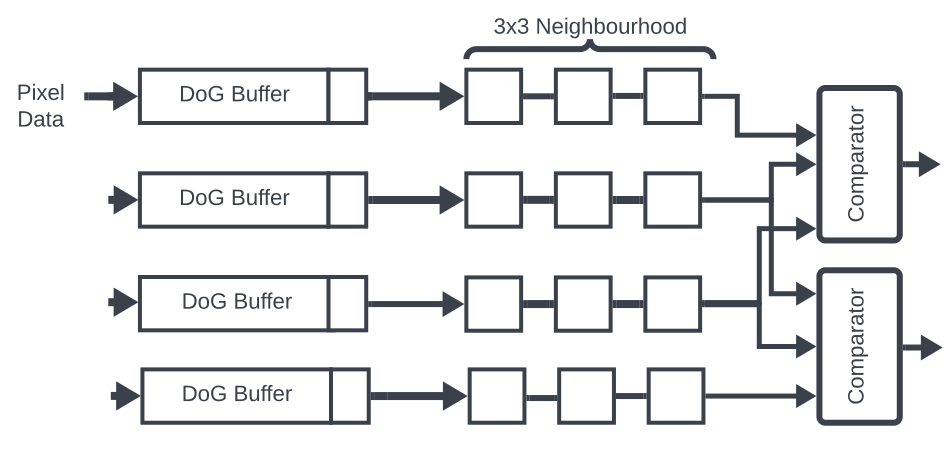
\includegraphics[width=0.8\columnwidth]{Images/Extrema.png}
    \caption{Extrema Detection Module Block Diagram.}
    \label{fig:ExtremaHW}
\end{figure}


Subsequently, adjacent levels of the Gaussian pyramid are subtracted from each other to obtain the DoG pyramid. This subtraction operation is preformed in parallel between each scale and the three resulting  DoG are buffered. Two row buffers are used for every DoG and form a $3 \times 3$ neighbourhood for extrema detection. \Fig{ExtremaHW} illustrates the design of maxima detector module where each pixel is then compared to its 26 neighbors, and the minimum magnitude is computed to determine the local extremum. Each DoG buffers output consists of three values that constitute one column of a 3x3 neighbouring window. The DoG words are forwarded to a comparator circuit which compares the middle pixel of DoG2 with its neighbours, and an OR gate indicates if it's an extremum. Note that the first row is processed on the fly without requiring buffers, since DoG operation is a single-pixel operation and doesn't affect the boundaries. The width of these buffers depends on the range of the DoG operation results.




\textbf{CORDIC \& Prewitt Mask Module:}
\begin{figure}[h]
    \centering
     \includegraphics[width=0.8\columnwidth]{Images/CORDIC.png}
    \caption{CORDIC Module Block Diagram. \cite{AMD12}}
    \label{fig:CORDIC}
\end{figure}

In the proposed implementation, the first derivatives of G2, are produced by applying Prewitt mask operator to generates the first-order derivatives of the image with respect to both the x and y directions. The magnitude is efficiently computed using the sum of absolute values of \( G_x^2 \) and \( G_y^2 \). This approach replaces the square root operation traditionally used in gradient magnitude calculations. After computation, the result is stored as 8 bits, retaining only the integer part of the magnitude for subsequent calculations. The gradient orientation is computed traditionally by using large Look-Up Tables (LUTs) for precomputed arctangents and hardware resources for division operations. However, the implementation uses Xilinx IP CORDIC module, which solves trigonometric equations iteratively and also computes a broader range of equations, including the hyperbolic and square root. The output orientation assignments are stored as a 6-bit integers.


\textbf{Histogram \& Normalisation Module:}

In the SIFT descriptor generation stage, each keypoint contributes to histogram entries representing gradient orientations and magnitudes within a local region. Keypoints may influence multiple orientation bins, leading to limited parallelisation. To address this, the descriptor computation utilises eight BRAMs, each dedicated to a specific orientation bin. These arrays independently accumulates data from keypoints associated with a particular orientation, enabling parallel processing. Keypoint coordinates and orientation information are used to distribute magnitude contributions across the arrays. The non-data dependent nature of each array allows for pipelined accumulation and simultaneous processing of multiple keypoints. After processing all the keypoints, an adder tree sums histogram values stored in the array. 



\begin{figure}[h]
    \centering
     \includegraphics[width=0.8\columnwidth]{Images/Descriptor Gen.png}
    \caption{Descriptor Normalisation Block Diagram}
    \label{fig:Descriptorgenblock}
\end{figure}

The unnormalised histogram data is streamed into the final module shown in \Fig{Descriptorgenblock} that performs normalisation. The input data is converted into floating point representation, to ensure accuracy and comparability with other hardware architectures. Once, converted the data is stored into BRAM and L1-norm of the histogram is calculated concurrently using DSPs. Each entry in the histogram is subsequently divided by the computed L1-norm, followed by a square root operation. The resulting normalised values are then converted from floating-point to fixed-point representation (8 bit) to minimise storage space. Furthermore, the outputs from each processing element are accumulated into a unified output vector using a combination of FIFO buffers and a multiplexer.



\subsection{Digital Filters}
\begin{figure}[h]
\centering
\subfloat[Box]{\label{4figs-a}   
\(
    \begin{bmatrix}    
    1 & 1 & 1 \\
    0 & 0 & 0 \\
    -1 & -1 & -1 \\
    \end{bmatrix}
\)
}
\hfill
\subfloat[Gaussian]{\label{4figs-b} 
\(
  \frac{1}{16}
  \begin{bmatrix}    
    1 & 2 & 1 \\
    2 & 4 & 2 \\
    1 & 2 & 1 \\
  \end{bmatrix}
\)
}%
\hfill
\subfloat[Sobel X \& Y]{\label{4figs-c} 
\(
    \begin{bmatrix}    
    1 & 1 & 1 \\
    0 & 0 & 0 \\
    -1 & -1 & -1 \\
    \end{bmatrix}
\)
\(
    \begin{bmatrix}    
    1 & 0 & -1 \\
    1 & 0 & -1 \\
    1 & 0 & -1 \\
    \end{bmatrix}
\)
}%
\caption{Example approximated $3\times3$ image filter kernels.}
\label{fig:filter-kernels}
\end{figure}


Digital filters are a tool in image processing to extract useful information from noisy signals. They are commonly used for tasks such as smoothing, edge detection, and feature extraction. Filters operate by applying a kernel, or a small matrix of values, to each pixel of an image. The kernel is convolved with the image, and the resulting output value is placed in the corresponding pixel location of the output image shown in the \Eq{kernel}. $I(x,y)$ is the input image and $K(k_x,k_y)$ is the kernel. The convolution result $O(x,y)$ is calculated by:  

\begin{equation}\label{eq:kernel}
\begin{aligned}
O(x, y) &= \sum_{k_x} \sum_{k_y} I(x - k_x, y - k_y) \cdot K(k_x, k_y)
\end{aligned}
\end{equation}

The indices $k_x$ and $k_y$ correspond to the coordinates of the kernel $K$, $x$ and $y$ correspond to the coordinates of the output image $O$. 

% \subsubsection*{Box:}

% The box filter is a spatial smoothing technique that convolves the image with the kernel shown in \ref{4figs-a}, replacing each pixel value with the average of its neighbouring pixels. The kernel's size determines the extent of the neighbourhood considered for averaging. This process has the effect of reducing high frequency noise while preserving the edges and important details of the image. In,\Eq{box}, $B(i, j)$ denotes the output intensity value at pixel location $(i, j)$ after applying the box filter. The filter's size is controlled by the parameter $A$, which is the total number of pixels within the filter's neighbourhood. The summation terms with indices $m$ and $n$ iterate over each pixel within the filter's rectangular neighbourhood, defined by a radius $r$ around the central pixel $(i, j)$.

% \begin{equation}\label{eq:box}
% B(x, y) = \frac{1}{A} \sum_{m=-r}^{r} \sum_{n=-r}^{r} A(x+m, y+n)
% \end{equation}

%  The box filter is also computationally efficient and easy to implement, making it a popular choice for many image processing applications. However, larger kernel sizes may cause blurring and loss of sharpness in the image.




% \subsubsection*{Gaussian:}
% The Gaussian filter is a widely used linear filter in image processing and computer vision. It is a type of low-pass filter that removes high-frequency noise while preserving the edges in an image. The filter works by convolving the image with a Gaussian kernel in \ref{4figs-b}, which is a normalised two-dimensional Gaussian distribution. The Gaussian kernel has a circularly symmetric shape and can be expressed mathematically as:

% \begin{equation}
% G(x,y) = \frac{1}{2\pi\sigma^2} e^{-\frac{x^2+y^2}{2\sigma^2}}
% \end{equation}

% where $\sigma$ is the standard deviation of the Gaussian distribution, and $x$ and $y$ are the distances from the centre of the kernel. The size of the kernel and the value of $\sigma$ determine the amount of smoothing applied to the image.


% \subsubsection*{Sobel:}
% The Sobel filter is a type of edge-detection filter that uses two kernels shown in \ref{4figs-c}, one for horizontal changes ( x kernel) and one for vertical changes ( y kernel) in an image. The Sobel filter works by convolving each of these kernels with the image and then computing the gradient magnitude at each pixel using the formula:

% \begin{equation}
% \sqrt{(G_x^2 + G_y^2)}
% \end{equation} 

% where $G_x$ and $G_y$ are the convolved images using the x and y kernels, respectively. The resulting gradient image highlights edges in the original image, and the direction of the edge can be determined by calculating the angle of the gradient using:

% \begin{equation}
% \theta = \tan^{-1}(G_y / G_x)
% \end{equation} 


\subsection{Convolutional Neural Network}\label{sec:CNN}

\begin{figure}[!h]
    \centering
     \includegraphics[width=\linewidth]{Images/CNN.png}
    \caption{Typical layers implemented within CNN Architectures.}
    \label{fig:CNN}
\end{figure}




Convolutional Neural Networks are a class of deep neural networks typically applied to images to recognise and classify particular features. A CNN architecture typically consists of a combination of convolution, pooling, and fully connected layers shown in \Fig{CNN}.

The convolution layers extract features by applying a convolution operation to the input image using a set of learnable filters (also called kernels or weights) designed to detect specific features. The output of the convolution operation is a feature map, which is then passed through a non-linear activation function, such as ReLU, to introduce non-linearity into the network. The convolutional layers can be stacked to form a deeper architecture, where each layer is designed to detect more complex features than the previous one. In addition, it is the most computationally intensive layer because each output element in the feature map is computed by repeatedly taking a dot product between the filter and a local patch of the input, which results in a large number of multiply-add operations.

The pooling layers are responsible for reducing the spatial size of the feature maps while retaining important information. The most common types of pooling are max pooling and average pooling. These layers typically use a small window that moves across the feature map and selects the maximum or average value within the window. This operation effectively reduces the number of parameters in the network and helps to reduce overfitting.

The fully connected layers make predictions based on the extracted features. These layers take the output from the convolutional and pooling layers and apply a linear transformation to the input, followed by a non-linear activation function. The fully connected layer usually has the same number of neurons as the number of classes in the dataset, and the output of this layer is passed through a softmax activation function to produce probability scores for each class.
A CNN architecture also includes normalisation layers such as batch normalisation, dropout layers that are used to regularise the network and reduce overfitting, and an output layer that produces the final predictions.

 

\section{Experimental Results and Discussion} \label{sec:result}
%--------------------------------------------------
\begin{table}
\centering
\setlength{\extrarowheight}{0pt}
\addtolength{\extrarowheight}{\aboverulesep}
\addtolength{\extrarowheight}{\belowrulesep}
\setlength{\aboverulesep}{0pt}
\setlength{\belowrulesep}{0pt}
\caption{Summary Table: Hardware/Software Environment \& Measurement Tools}
\label{tab:HWEnvironment}
\arrayrulecolor{black}
\resizebox{\linewidth}{!}{%
\begin{tabular}{c|c|c|c|c} 
\toprule
\rowcolor[rgb]{0.753,0.753,0.753} {\cellcolor[rgb]{0.753,0.753,0.753}} & \multicolumn{2}{c|}{Hardware} & {\cellcolor[rgb]{0.753,0.753,0.753}} & \multicolumn{1}{c|}{{\cellcolor[rgb]{0.753,0.753,0.753}}} \\ 
\hhline{>{\arrayrulecolor[rgb]{0.753,0.753,0.753}}->{\arrayrulecolor{black}}|-|-|>{\arrayrulecolor[rgb]{0.753,0.753,0.753}}->{\arrayrulecolor{black}}|>{\arrayrulecolor[rgb]{0.753,0.753,0.753}}->{\arrayrulecolor{black}}|}
\rowcolor[rgb]{0.753,0.753,0.753} \multirow{-2}{*}{{\cellcolor[rgb]{0.753,0.753,0.753}}Architecture} & Model & Clock & \multirow{-2}{*}{{\cellcolor[rgb]{0.753,0.753,0.753}}Software /Libraries} & \multicolumn{1}{c|}{\multirow{-2}{*}{{\cellcolor[rgb]{0.753,0.753,0.753}}\begin{tabular}[c]{@{}>{\cellcolor[rgb]{0.753,0.753,0.753}}c@{}}Power\\ Measurement\end{tabular}}} \\ 
\cmidrule{1-3}\cline{4-4}\cmidrule{5-5}
CPU & AMD 5900x & 4.8 GHz & \multicolumn{1}{l|}{Pytorch 2.0\cite{Pytorch} / OpenCV} & HWMonitor\cite{cpuid} \\ 
\cmidrule{1-1}\cline{2-5}
GPU & Nvidia GTX 3070 & 1730 MHz & Pytorch 2.0 / OpenCV & Nvidia-smi\cite{Nvidiasmi} \\ 
\cmidrule{1-2}\cline{3-5}
FPGA & Xilinx ZCU102 & 300Mhz & \begin{tabular}[c]{@{}c@{}}Vivado 2022.2 / \\Vitis 2020.2\end{tabular} & \begin{tabular}[c]{@{}c@{}}MaxPower-tool\cite{MAXIM} / \\Power Analyser\end{tabular} \\
\bottomrule
\end{tabular}
}
\end{table}
%\vspace{-10mm}
%--------------------------------------------------


\begin{figure}[!h]
    \centering
     \includegraphics[width=\columnwidth]{Images/FilterAlgorithms.png}
    \caption{Filter Algorithms Applied onto Input Image}
    \label{fig:FilterAlgorithms}
\end{figure}

We verify the proposed optimisations on 'SIFT', 'Box', 'Gaussian' and 'Sobel' (in \Fig{FilterAlgorithms}) algorithms, as well as MobileNetV2 and ResNet50 CNN architectures. This is achieved by creating baseline benchmarks on four target hardware CPU, GPU and FPGA, followed by the realisations of the optimisations individually and combined. The CPU and GPU versions for Filter and SIFT algorithms are implemented using \textit{OpenCV}\cite{opencv_library}. Pytorch library is used to implement CNN architectures (ResNet50 \& MobileNetV2) and optimisations. Additionally, both architectures are pre-trained on the image-net classification dataset. The FPGA implementation for all algorithms is developed using Verilog (SIFT/Filter) and HLS (CNN). All baseline algorithms and CNN models use floating point 32 (FP32), and an uncompressed grayscale $8$-bit $1920\times1080$ input image is used for the SIFT algorithm, and each sub-operation is profiled. Details of the target hardware/software environments and power measurement tools are given in \Tab{HWEnvironment}. 

\textbf{Dataset.} The input images used in the CNN and Filter experiments are from LIU4K-v2 dataset \cite{LiuliuYan19}. The dataset contains 2000 high resolution $3840\times2160$ images with various backgrounds and objects. 

\subsection{Performance Metrics}

As part of the evaluation process, we measure three different performance metrics, namely, \textit{1) execution time}, \textit{2) energy consumption} and \textit{3) accuracy}.

\subsubsection{Execution time}
The execution time measured for the CPU and GPU platforms uses time function libraries to count the smallest tick period. Each algorithm/operation is run for 1000 iterations and averaged to minimise competing resources or other processes directly affecting the architecture, especially for the CPU architecture. The GPU has an initialisation time which is taken into account and removed from the results. The timing simulation integrated into Vivado design suite software is used to measure the time for the FPGA platform. The experiments exclude the time of both the image read and write from external memory. We compute the frame per second (FPS) as the inverse of the execution time: 
\begin{equation}\label{eq:FPS}
\text{FPS}= 1/\text{Execution Time}.
\end{equation}

\subsubsection{Power Consumption}
Two common methods used for measuring power are software and hardware-based. Accurately estimating power consumption is a challenge using software-based methods, which have underlying assumptions in their models and may not measure other components within the platform. In addition, taking the instantaneous watt or theoretical TDP of a device is not accurate since power consumption varies on the specific workload. Therefore, we obtain the total energy consumed by measuring the power over the duration of the algorithm executed. A script is developed to start and stop the measurements during the execution of the algorithm and extract the power values from the software. 

With the use of a power analyser within the Vivado design suite and the MaxPower-tool, the measurement of FPGA power consumption is divided into two parts, \textit{(1)}~static power and \textit{(2)}~dynamic power. Static power relates to the consumption of power when there is no circuit activity and the system remains idle. Dynamic power is the power consumed when the design is actively performing tasks. The power consumption for the CPU and GPU is obtained using \textit{HWMonitor} and \textit{Nvidia-smi} software.
To have a fair comparison across the target hardware for the SIFT algorithm, we normalise it as the energy per operation (EPO):
%------------------------------------------
\begin{equation}\label{eq:energy1}
\text{Energy} = (\text{Power} * \text{Execution Time}).    
\end{equation}

Additionally, We calculate the energy consumption for the Filter and CNN algorithms:

\begin{equation}\label{eq:energy}
\text{EPO} = (\text{Power} * \text{Execution Time})/\text{Operations}.    
\end{equation}


%------------------------------------------

%In this paper, we focused on implementing and evaluating a commonly used feature extraction algorithm named SIFT. Initially, an OpenCV SIFT algorithm is profiled on the CPU/GPU to analyse the hot spots and characteristics. Secondly, domain-specific optimisation strategies are applied to the FPGA implementation such as resizing the convolution filter, down-sampling, bit-width and integer arithmetic. These optimisations were also applied together in various combinations to see if one optimisation affected another in performance.

%We provide metrics to understand which optimisations perform well on the FPGA implementation. For each optimisation of the SIFT algorithm, we measure the execution time on each/group of optimisations to determine which optimisation executed the floating-point / integer operation in the least amount of time.

\subsubsection{Accuracy}

With an expectation that the optimisations impact overall algorithmic accuracy, we capture it by measuring the \textit{Euclidean distance} between the descriptors generated from the CPU (our comparison benchmark) to the descriptor output produced by the FPGA. The Euclidean distance $d(x,y)$ is calculated in \Eq{Euc} where $x$ and $y$ are vectors, and $K$ is the number of keypoints generated. This accuracy measurement is only used for the SIFT algorithm implementation.

%-------------------------------
\begin{equation}\label{eq:Euc}
d(x,y)=\sqrt{\sum_{i=1}^{K} (x_{i}-y_{i})^{2}}.
\end{equation}

Subsequently, the accuracy for each Euclidean distance is calculated using \Eq{Accu}:
\begin{equation}\label{eq:Accu}
\text{Accuracy} = 100 - \left( \left( \frac{\text{Euclidean Distance}}{\text{Max Distance}} \right) \times 100\right)
\end{equation}

The \textit{Euclidean Distance} denotes the distance between the two descriptor vectors being compared, and \textit{Max Distance} represents the maximum Euclidean distance found in the vector. The accuracy is transformed to have 100\% indicate identical descriptors, while 0\% indicates completely dissimilar descriptors.

We used root mean square error (RSME) to compare the input image to the output images produced by each hardware accelerator to determine the pixel accuracy. RMSE is defined as:
\begin{equation}
RMSE = \sqrt{(\frac{1}{n})\sum_{i=1}^{n}(y_{i} - x_{i})^{2}}
\end{equation}
Where the difference between the pixel intensity values of output and input (y\textsubscript{i},x\textsubscript{i}) images. Divided by N, which is the total number of pixels in the image.\par


The accuracy of the CNN architecture is measured by taking the number of correct predictions divided by the total number of predictions:

\begin{equation}
\text{Accuracy} = \frac{\text{Number of Correct Predictions}}{\text{Total Number of Predictions}} \times 100
\end{equation}

A high accuracy indicates that the model is making accurate predictions, while a low accuracy suggests room for improvement in the model's performance. 






%-------------------------------

%-------------------------------

%------------------------------------

\subsection{Results and Discussions}
The results and discussions section contains the evaluation of algorithms in three categories, feature extraction algorithms (\textit{SIFT}), filter algorithms (\textit{Box, Gaussian, Sobel}) and Convolution Neural Networks (\textit{MobilenetV2, ResNet50}). 

\begin{table}[!h]
\caption{SIFT: Performance against state-of-the-art}
\label{tab:state_of_art}
\resizebox{\columnwidth}{!}{%
\begin{tabular}{lclrrr}
\toprule
 &
  \begin{tabular}[c]{@{}c@{}}Octave,\\ Scale\end{tabular} &
  Hardware Platform &
  Image Size &
  \begin{tabular}[c]{@{}c@{}}Clock\\ (Mhz)\end{tabular} &
  \begin{tabular}[c]{@{}r@{}}Frame Rate\\ (FPS)\end{tabular} \\ \midrule
Chiu~\cite{ChiTiaJiu13}     & 2,4 & Virtex-6           & $640\times480$     & 100 & 30  \\
Mizuno~\cite{MizKosNog11}   & 2,4 & 65 nm CMOS         & $1920\times1080$   & N/A  & 30  \\
Vourvoulakis~\cite{VourKalLy16}  & 1,4          & Cyclone IV        & $640\times480$  & 21.7   & 70  \\ \midrule
Proposed & 2,4 & Zynq UltraScale+   & $1920\times1080$ & 300 & 50  \\
 & 2,4 & Virtex UltraScale+ & $1920\times1080$ & 600 & \textbf{100}  \\ \bottomrule
\end{tabular}%
}
\end{table} 


%\subsection{Frames Per Second \& Accuracy}
\subsubsection{SIFT}

\begin{figure}[h]
    \centering
\resizebox{\columnwidth}{!}{\pgfplotsset{
  my axis style/.style={
      width=\linewidth,
      ybar=2*\pgflinewidth,
      ybar=5pt,
      bar width=0.50cm,
      enlarge y limits=0.0,
      enlarge x limits=0.10,
      xticklabels from table={\data}{material},
      xtick={data},
      table/x expr={\coordindex},
      xtick align=inside,
      xticklabel style={align=center},
      %minor y tick num=1,
      scaled y ticks=false,
      yticklabel style={/pgf/number format/fixed},
    },
  Name/.style={
      nodes near coords,
      nodes near coords style={
          coordinate,
          name=#1\coordindex,
          mark=*, % add red circle at node
          mark options={mark size=2pt, fill=red}, % set size and fill color of mark
        },
    },
}

\pgfplotstableread{
  material d1 d2 T1 T2 
  Base\\FPGA 23.26 10.7 98.82 99.34 
  3X3\\Krnl 33.33 11.23 97.34 98.98 
  Dsp\\(1/2) 37.04 13.15 95.24 97.62 
  Int         40 13.51 93.45 95.86 
  3x3\\+Int 43.48 15.15 93.34 94.45 
  Dsp\\+3X3 41.67 14.70 91.85 93.26
  Dsp\\+Int 45.45 15.87 90.78 91.52 
  Dsp\\+3X3\\+Int 50 16.67 89.45 90.18 
}{\data}

\begin{tikzpicture}
  \begin{axis}[    
  my axis style,       
  legend image code/.code={\draw[#1, 
  draw=none, fill=none] (0cm,-0.1cm) rectangle (0.3cm,0.25cm);
        },    
        ymin=0,
        ymax=80,  
        %ytick={0, 0.1, 0.2, 0.3, 0.4, 0.5, 0.6},
        legend columns=-1,
        nodes near coords,
        nodes near coords style={font=\small, anchor=west,rotate=90,inner xsep=0.5pt},
        axis x line*=bottom,      
        axis y line*=left,  
        ylabel=Frames Per Second (FPS),
      cycle list={
          {draw=black, fill=blue!20,},
          {draw=black, fill=red!20,},
        },
      scaled y ticks=false,
    ]
    \addplot table [y=d1] {\data};
    \addplot table [y=d2] {\data};
    %\legend{{Baseline}, {Datatype}}
  \end{axis}

  \begin{axis}[       
  my axis style,  
  legend style={at={(0.5,-0.12)},
          anchor=north,legend columns=-1},    
          ymin=60,   
          ymax=100,   
          axis y line*=right,  
          ylabel=Accuracy (\%),      
          xticklabels=\empty,      
          only marks,    
          scaled y ticks=false, 
          xtick = data,
        nodes near coords,
        nodes near coords style={font=\small, anchor=north,rotate=90,inner xsep=0.5pt},
    ]
\addplot [Name=a] table [y=T1, meta=T1] {\data};
\addplot [Name=b] table [y=T2, meta=T2] {\data};
\legend{{\color{blue!50}\rule{5mm}{2mm} \textcolor{black}{Octave/Scale: 2-4}}, {\color{red!50}\rule{5mm}{2mm} \textcolor{black}{Octave/Scale: 4-5}}}
\end{axis}

  \foreach \i in {0,1,2,3,4,5,6,7} {
      % \fill [red!90] (d\i) circle (2pt);
      \fill [blue!90] (a\i) circle (2pt);
      % \draw [very thick,red!90] (d\i) -- (e\i) -- (f\i);
      % \draw [very thick,blue!90] (a\i) -- (b\i) -- (c\i);
      % \fill [red!90] (e\i) circle (2pt);
      % \fill [red!90] (f\i) circle (2pt);
      \fill [red!90] (b\i) circle (2pt);
      % \fill [blue!90] (c\i) circle (2pt);
    }

\foreach \i in {0,1,2,3,4,5,6,7} {
  \ifnum\i=0
    \fill [red!90] (b\i) circle (2pt) node[below] {\pgfplotstablegetelem{\i}{[index]4}\of{\data}\pgfplotsretval};
    \fill [blue!90] (a\i) circle (2pt) node[below, rotate=-45] {\pgfplotstablegetelem{\i}{[index]3}\of{\data}\pgfplotsretval};
  \else
    \ifnum\i=1
      \fill [red!90] (b\i) circle (2pt) node[below] {\pgfplotstablegetelem{\i}{[index]4}\of{\data}\pgfplotsretval};
    \else
      \fill [red!90] (b\i) circle (2pt) node[above] {\pgfplotstablegetelem{\i}{[index]4}\of{\data}\pgfplotsretval};
    \fi
    \fill [blue!90] (a\i) circle (2pt) node[below] {\pgfplotstablegetelem{\i}{[index]3}\of{\data}\pgfplotsretval};
  \fi
}



\end{tikzpicture}}    %\caption{Execution times for individual and combined algorithms.}
    %\vspace{-6mm}
    \caption[SIFT: FPS and Accuracy]{SIFT: FPS (Bars) and Accuracy (Dots) for each optimisation on both configurations (octave, scale).}
    %\vspace{-3mm}
    \label{fig:ResAccGraph}
\end{figure}

We obtain results for FPGA implementations of the SIFT algorithm, considering various optimisations or combinations of them. Two sets of results are captured for \textit{octave, scale} of (2,4) and (4,5) as they are regularly reported in the literature for SIFT implementation on FPGA. The results are primarily obtained at a target frequency of 300 MHz for various components of SIFT and execution time and accuracy are reported in \Tab{Optimisation_Summary} along with FPS numbers in \Fig{ResAccGraph}. 

In terms of individual optimisations on the base FPGA implementation, \textit{down sampling} and \textit{integer} optimisations had the most reduction of accuracy but in trade for a greater reduction of runtime. On the other hand, \textit{$3\times3$ kernel size} (down from default $5\times 5$) had better accuracy results but with a small improvement on the overall runtime. In the case of combined optimisations, both \textit{down sampling} and \textit{integer} combinations greatly reduced the execution times but at a cost of $8\sim10\%$ accuracy loss. In the most optimised case, (4,5) and (2,4) configurations achieved $17$ and $50$ fps, at an accuracy of $90.18\%$ and $89.45\%$, respectively. The $10 \sim 11\%$ loss in accuracy in both configurations can be attributed to the loss of precision and pixel information resulting in imperfection in feature detection.

The comparison with optimised CPU and GPU implementations is shown in  \Tab{platoformsummary} which includes total execution time and energy consumption per operation (nJ/Op). Results indicate the optimised FPGA implementation achieved comparable GPU runtime at 600 MHz but significantly outperformed them when energy consumption statistics are taken into account. The GPU results excluded the initialisation time, which would add greater latency to the overall runtime. In addition, the power consumption of the GPU is at $12.47$nJ/Op, which would make it a difficult choice for real-time embedded systems. On the other hand, optimised FPGA implementations have better performance per watt than the GPU and CPU. The comparison with the state-of-the-art FPGA implementations is reported in \Tab{state_of_art}, and results show major improvements in the runtime even with larger image size and more or similar feature points ($\sim10000$). Finally, for completeness, we report the resource and power usage statistics for optimised configurations at 300 MHz in \Tab{resourseusage}.


 \subsubsection{Filter Implementations}
\begin{figure}[!h]
    \centering
\resizebox{\columnwidth}{!}{\begin{tikzpicture}
    \begin{axis}[   
    width  = \textwidth,    
    major x tick style = transparent,   
    ybar=2*\pgflinewidth,     
    ymin=0,       
    bar width=6.5pt,      
    enlarge y limits={upper=0.15},    
    legend image code/.code={\draw[#1, draw=none, fill=none] (1cm,-0.1cm) rectangle (0.3cm,0.3cm);
                },
        ymajorgrids = true,
        xticklabel style={font=\bfseries},
        ylabel style={font=\bfseries},
        ylabel = {Execution Time (ms)},
        extra y ticks={0},       
        symbolic x coords={Baseline,Datatype,3X3 Kernel,Dwnsmple,Separable}, 
        xtick = data,
        nodes near coords,
        nodes near coords style={font=\small, anchor=west,rotate=90,inner xsep=0.5pt},
        scaled y ticks = false,
        enlarge x limits=0.15,
        legend cell align=left,
        enlarge y limits={upper=0.15},
        legend style={at={(0.56,1.6)}, anchor=west, legend columns=-1, font=\large}
    ]
        \addplot[draw=black, pattern=north east lines, pattern color=black, postaction={pattern=north east lines}, fill=blue!40] coordinates {(Baseline, 14) (Datatype,12) (3X3 Kernel,8)(Dwnsmple,10)(Separable,6)}; % Changed this line
        
        \addplot[draw=black, pattern=north east lines, pattern color=black, postaction={pattern=north east lines},fill=green!40] coordinates {(Baseline,2.9) (Datatype,2.6) (3X3 Kernel,2.1)(Dwnsmple,2.4)(Separable,1.5)}; % Changed this line
        
        \addplot[draw=black, pattern=north east lines, pattern color=black, postaction={pattern=north east lines},fill=red!40] coordinates {(Baseline,3.2) (Datatype,2.9) (3X3 Kernel,2.3)(Dwnsmple,2.5)(Separable,1.8)}; % Changed this line
        
        \addplot[draw=black, pattern=crosshatch, pattern color=black, postaction={pattern=crosshatch}, fill=blue!40]  coordinates {(Baseline, 12) (Datatype,10) (3X3 Kernel,6)(Dwnsmple, 8)(Separable,4)}; % Changed this line
        
       \addplot[draw=black, pattern=crosshatch, pattern color=black, postaction={pattern=crosshatch},fill=green!40] coordinates {(Baseline,2.3) (Datatype,1.9) (3X3 Kernel,1.5)(Dwnsmple,1.8) (Separable,1.1)}; % Changed this line
       
        \addplot[draw=black, pattern=crosshatch, pattern color=black, postaction={pattern=crosshatch},fill=red!40] coordinates {(Baseline,2.5) (Datatype,2.1) (3X3 Kernel,1.6)(Dwnsmple,1.9) (Separable,1.3)}; % Changed this line
        
        \addplot[draw=black, pattern=horizontal lines, pattern color=black, postaction={pattern=horizontal lines}, fill=blue!40]  coordinates {(Baseline, 30) (Datatype,27) (3X3 Kernel,23)(Dwnsmple,25) (Separable,15)}; % Changed this line
        
        \addplot[draw=black, pattern=horizontal lines, pattern color=black, postaction={pattern=horizontal lines},fill=green!40] coordinates {(Baseline,3.4) (Datatype,3.1) (3X3 Kernel,2.7)(Dwnsmple,2.9) (Separable,1.8)}; % Changed this line
        
        \addplot[draw=black, pattern=horizontal lines, pattern color=black, postaction={pattern=horizontal lines},fill=red!40] coordinates {(Baseline,3.2) (Datatype,2.9) (3X3 Kernel,2.4)(Dwnsmple,2.7)(Separable,1.6)}; % Changed this line
    \end{axis}

\begin{axis}[hide axis,
extra y ticks={0},     
xmin=0,
xmax=1,
ymin=0,
ymax=1,
legend style={at={(0.54,-0.30)}, anchor=west, legend columns=-1, font=\large}]    
    \addlegendimage{legend image code/.code={\draw[#1, draw=none] (0cm,-0.1cm) rectangle (0.3cm,0.1cm);}, legend image post style={line width=1.5pt}}    
    \addlegendentry{}    
    \addlegendimage{blue!40, line width=5pt}    
    \addlegendentry{CPU}
    \addlegendimage{green!40, line width=5pt}    
    \addlegendentry{GPU}
    \addlegendimage{red!40, line width=5pt}    
    \addlegendentry{FPGA}    
\end{axis}

\begin{axis}[
    hide axis,
    xmin=0,
    extra y ticks={0},     
    xmax=1,
    ymin=0,
    ymax=1,
    xticklabels={Baseline,DataType,3x3 Kernel, Separable},
    legend style={
        at={(0.9,1.9)},
        anchor=west,
        legend columns=-1,
        font=\large
    },
    legend image code/.code={\draw[#1,  fill=none] (1cm,-0.1cm) rectangle (0.3cm,0.3cm);
                }
]
    \addplot[
        draw=none,
        pattern=north east lines,
        pattern color=black,
        postaction={pattern=north east lines},
        fill=blue!40
    ] coordinates {
        (0, 0)
        (0, 0)
        (0, 0)
    };
        
    \addplot[
        draw=none,
        pattern=crosshatch,
        pattern color=black,
        postaction={pattern=crosshatch},
        fill=green!40
    ] coordinates {
        (0,0)
        (0,0)
        (0,0)
    };
        
    \addplot[
        draw=none,
        pattern=horizontal lines,
        pattern color=black,
        postaction={pattern=horizontal lines},
        fill=red!40
    ] coordinates {
        (0,0)
        (0,0)
        (0,0)
    };
    
    \legend{Box,Gaussian,Sobel}
\end{axis}

\end{tikzpicture}
}    %\caption{Execution times for individual and combined algorithms.}
    %\vspace{-6mm}
    \caption[Filter: Runtime comparison for optimisations]{Filter: Runtime comparison for optimisations applied on each architecture.  }
    \label{fig:FilterRuntime}
\end{figure}


\begin{figure}[!h]
    \centering
\resizebox{\columnwidth}{!}{\begin{tikzpicture}
    \begin{axis}[   
    width  = \textwidth,    
    major x tick style = transparent,   
    ybar=2*\pgflinewidth,     
    ymin=0,       
    bar width=6.5pt,      
    enlarge y limits={upper=0.15},    
    legend image code/.code={\draw[#1, draw=none, fill=none] (1cm,-0.1cm) rectangle (0.3cm,0.3cm);
                },
        ymajorgrids = true,
        xticklabel style={font=\bfseries},
        ylabel style={font=\bfseries},
        ylabel = {Energy Consumption (Joules)},
        extra y ticks={0},       
        symbolic x coords={Baseline,Datatype,3X3 Kernel,Dwnsmple,Separable}, 
        xtick = data,
        nodes near coords,
        nodes near coords style={font=\small, anchor=west,rotate=90,inner xsep=0.5pt,  /pgf/number format/.cd,  fixed, precision=2},
        scaled y ticks = false,
        enlarge x limits=0.15,
        legend cell align=left,
        enlarge y limits={upper=0.15},
        legend style={at={(0.56,1.6)}, anchor=west, legend columns=-1, font=\large}
    ]
        \addplot[draw=black, pattern=north east lines, pattern color=black, postaction={pattern=north east lines}, fill=blue!40] coordinates {(Baseline, 1.12) (Datatype,1.03) (3X3 Kernel,0.6)(Dwnsmple,0.95)(Separable,0.56)}; % Changed this line
        
        \addplot[draw=black, pattern=north east lines, pattern color=black, postaction={pattern=north east lines},fill=green!40] coordinates {(Baseline,0.10) (Datatype,0.08) (3X3 Kernel,0.04)(Dwnsmple,0.10)(Separable,0.08)}; % Changed this line
        
        \addplot[draw=black, pattern=north east lines, pattern color=black, postaction={pattern=north east lines},fill=red!40] coordinates {(Baseline,0.08) (Datatype,0.07) (3X3 Kernel,0.05)(Dwnsmple,0.075)(Separable,0.06)}; % Changed this line
        
        \addplot[draw=black, pattern=crosshatch, pattern color=black, postaction={pattern=crosshatch}, fill=blue!40]  coordinates {(Baseline, 0.91) (Datatype,0.78) (3X3 Kernel,0.50)(Dwnsmple, 0.70)(Separable,0.36)}; % Changed this line
        
       \addplot[draw=black, pattern=crosshatch, pattern color=black, postaction={pattern=crosshatch},fill=green!40] coordinates {(Baseline,0.09) (Datatype,0.06) (3X3 Kernel,0.07)(Dwnsmple,0.08) (Separable,0.044)}; % Changed this line
       
        \addplot[draw=black, pattern=crosshatch, pattern color=black, postaction={pattern=crosshatch},fill=red!40] coordinates {(Baseline,0.06) (Datatype,0.05) (3X3 Kernel,0.04)(Dwnsmple,0.06) (Separable,0.041)}; % Changed this line
        
        \addplot[draw=black, pattern=horizontal lines, pattern color=black, postaction={pattern=horizontal lines}, fill=blue!40]  coordinates {(Baseline, 2.46) (Datatype,2.27) (3X3 Kernel,1.98)(Dwnsmple,2.32) (Separable,1.38)}; % Changed this line
        
        \addplot[draw=black, pattern=horizontal lines, pattern color=black, postaction={pattern=horizontal lines},fill=green!40] coordinates {(Baseline,0.12) (Datatype,0.11) (3X3 Kernel,0.095)(Dwnsmple,0.12) (Separable,0.10)}; % Changed this line
        
        \addplot[draw=black, pattern=horizontal lines, pattern color=black, postaction={pattern=horizontal lines},fill=red!40] coordinates {(Baseline,0.08) (Datatype,0.07) (3X3 Kernel,0.072)(Dwnsmple,0.078)(Separable,0.05)}; % Changed this line
    \end{axis}

\begin{axis}[hide axis,
extra y ticks={0},     
xmin=0,
xmax=1,
ymin=0,
ymax=1,
legend style={at={(0.58,-0.30)}, anchor=west, legend columns=-1, font=\large}]    
    \addlegendimage{legend image code/.code={\draw[#1, draw=none] (0cm,-0.1cm) rectangle (0.3cm,0.1cm);}, legend image post style={line width=1.5pt}}    
    \addlegendentry{}    
    \addlegendimage{blue!40, line width=5pt}    
    \addlegendentry{CPU}
    \addlegendimage{green!40, line width=5pt}    
    \addlegendentry{GPU}
    \addlegendimage{red!40, line width=5pt}    
    \addlegendentry{FPGA}    
\end{axis}

\begin{axis}[
    hide axis,
    xmin=0,
    extra y ticks={0},     
    xmax=1,
    ymin=0,
    ymax=1,
    xticklabels={Baseline,DataType,3x3 Kernel, Separable},
    legend style={
        at={(0.9,1.9)},
        anchor=west,
        legend columns=-1,
        font=\large
    },
    legend image code/.code={\draw[#1,  fill=none] (1cm,-0.1cm) rectangle (0.3cm,0.3cm);
                }
]
    \addplot[
        draw=none,
        pattern=north east lines,
        pattern color=black,
        postaction={pattern=north east lines},
        fill=blue!40
    ] coordinates {
        (0, 0)
        (0, 0)
        (0, 0)
    };
        
    \addplot[
        draw=none,
        pattern=crosshatch,
        pattern color=black,
        postaction={pattern=crosshatch},
        fill=green!40
    ] coordinates {
        (0,0)
        (0,0)
        (0,0)
    };
        
    \addplot[
        draw=none,
        pattern=horizontal lines,
        pattern color=black,
        postaction={pattern=horizontal lines},
        fill=red!40
    ] coordinates {
        (0,0)
        (0,0)
        (0,0)
    };
    
    \legend{Box,Gaussian,Sobel}
\end{axis}

\end{tikzpicture}
}    %\caption{Execution times for individual and combined algorithms.}
    %\vspace{-6mm}
    \caption[Filter: Energy consumption comparison]{Filter: Energy consumption comparison for optimisations applied on each architecture.}
    \label{fig:FilterEnergy}
\end{figure}

% \begin{figure}[h]
%     \centering
%     \begin{tabular}{cc}
%     \resizebox{0.46\linewidth}{!}{\begin{tikzpicture}
    \begin{axis}[   
    width  = \textwidth,    
    major x tick style = transparent,   
    ybar=2*\pgflinewidth,     
    ymin=0,       
    bar width=6.5pt,      
    enlarge y limits={upper=0.15},    
    legend image code/.code={\draw[#1, draw=none, fill=none] (1cm,-0.1cm) rectangle (0.3cm,0.3cm);
                },
        ymajorgrids = true,
        xticklabel style={font=\bfseries},
        ylabel style={font=\bfseries},
        ylabel = {Execution Time (ms)},
        extra y ticks={0},       
        symbolic x coords={Baseline,Datatype,3X3 Kernel,Dwnsmple,Separable}, 
        xtick = data,
        nodes near coords,
        nodes near coords style={font=\small, anchor=west,rotate=90,inner xsep=0.5pt},
        scaled y ticks = false,
        enlarge x limits=0.15,
        legend cell align=left,
        enlarge y limits={upper=0.15},
        legend style={at={(0.56,1.6)}, anchor=west, legend columns=-1, font=\large}
    ]
        \addplot[draw=black, pattern=north east lines, pattern color=black, postaction={pattern=north east lines}, fill=blue!40] coordinates {(Baseline, 14) (Datatype,12) (3X3 Kernel,8)(Dwnsmple,10)(Separable,6)}; % Changed this line
        
        \addplot[draw=black, pattern=north east lines, pattern color=black, postaction={pattern=north east lines},fill=green!40] coordinates {(Baseline,2.9) (Datatype,2.6) (3X3 Kernel,2.1)(Dwnsmple,2.4)(Separable,1.5)}; % Changed this line
        
        \addplot[draw=black, pattern=north east lines, pattern color=black, postaction={pattern=north east lines},fill=red!40] coordinates {(Baseline,3.2) (Datatype,2.9) (3X3 Kernel,2.3)(Dwnsmple,2.5)(Separable,1.8)}; % Changed this line
        
        \addplot[draw=black, pattern=crosshatch, pattern color=black, postaction={pattern=crosshatch}, fill=blue!40]  coordinates {(Baseline, 12) (Datatype,10) (3X3 Kernel,6)(Dwnsmple, 8)(Separable,4)}; % Changed this line
        
       \addplot[draw=black, pattern=crosshatch, pattern color=black, postaction={pattern=crosshatch},fill=green!40] coordinates {(Baseline,2.3) (Datatype,1.9) (3X3 Kernel,1.5)(Dwnsmple,1.8) (Separable,1.1)}; % Changed this line
       
        \addplot[draw=black, pattern=crosshatch, pattern color=black, postaction={pattern=crosshatch},fill=red!40] coordinates {(Baseline,2.5) (Datatype,2.1) (3X3 Kernel,1.6)(Dwnsmple,1.9) (Separable,1.3)}; % Changed this line
        
        \addplot[draw=black, pattern=horizontal lines, pattern color=black, postaction={pattern=horizontal lines}, fill=blue!40]  coordinates {(Baseline, 30) (Datatype,27) (3X3 Kernel,23)(Dwnsmple,25) (Separable,15)}; % Changed this line
        
        \addplot[draw=black, pattern=horizontal lines, pattern color=black, postaction={pattern=horizontal lines},fill=green!40] coordinates {(Baseline,3.4) (Datatype,3.1) (3X3 Kernel,2.7)(Dwnsmple,2.9) (Separable,1.8)}; % Changed this line
        
        \addplot[draw=black, pattern=horizontal lines, pattern color=black, postaction={pattern=horizontal lines},fill=red!40] coordinates {(Baseline,3.2) (Datatype,2.9) (3X3 Kernel,2.4)(Dwnsmple,2.7)(Separable,1.6)}; % Changed this line
    \end{axis}

\begin{axis}[hide axis,
extra y ticks={0},     
xmin=0,
xmax=1,
ymin=0,
ymax=1,
legend style={at={(0.54,-0.30)}, anchor=west, legend columns=-1, font=\large}]    
    \addlegendimage{legend image code/.code={\draw[#1, draw=none] (0cm,-0.1cm) rectangle (0.3cm,0.1cm);}, legend image post style={line width=1.5pt}}    
    \addlegendentry{}    
    \addlegendimage{blue!40, line width=5pt}    
    \addlegendentry{CPU}
    \addlegendimage{green!40, line width=5pt}    
    \addlegendentry{GPU}
    \addlegendimage{red!40, line width=5pt}    
    \addlegendentry{FPGA}    
\end{axis}

\begin{axis}[
    hide axis,
    xmin=0,
    extra y ticks={0},     
    xmax=1,
    ymin=0,
    ymax=1,
    xticklabels={Baseline,DataType,3x3 Kernel, Separable},
    legend style={
        at={(0.9,1.9)},
        anchor=west,
        legend columns=-1,
        font=\large
    },
    legend image code/.code={\draw[#1,  fill=none] (1cm,-0.1cm) rectangle (0.3cm,0.3cm);
                }
]
    \addplot[
        draw=none,
        pattern=north east lines,
        pattern color=black,
        postaction={pattern=north east lines},
        fill=blue!40
    ] coordinates {
        (0, 0)
        (0, 0)
        (0, 0)
    };
        
    \addplot[
        draw=none,
        pattern=crosshatch,
        pattern color=black,
        postaction={pattern=crosshatch},
        fill=green!40
    ] coordinates {
        (0,0)
        (0,0)
        (0,0)
    };
        
    \addplot[
        draw=none,
        pattern=horizontal lines,
        pattern color=black,
        postaction={pattern=horizontal lines},
        fill=red!40
    ] coordinates {
        (0,0)
        (0,0)
        (0,0)
    };
    
    \legend{Box,Gaussian,Sobel}
\end{axis}

\end{tikzpicture}
} &
%     \resizebox{0.46\linewidth}{!}{\begin{tikzpicture}
    \begin{axis}[   
    width  = \textwidth,    
    major x tick style = transparent,   
    ybar=2*\pgflinewidth,     
    ymin=0,       
    bar width=6.5pt,      
    enlarge y limits={upper=0.15},    
    legend image code/.code={\draw[#1, draw=none, fill=none] (1cm,-0.1cm) rectangle (0.3cm,0.3cm);
                },
        ymajorgrids = true,
        xticklabel style={font=\bfseries},
        ylabel style={font=\bfseries},
        ylabel = {Energy Consumption (Joules)},
        extra y ticks={0},       
        symbolic x coords={Baseline,Datatype,3X3 Kernel,Dwnsmple,Separable}, 
        xtick = data,
        nodes near coords,
        nodes near coords style={font=\small, anchor=west,rotate=90,inner xsep=0.5pt,  /pgf/number format/.cd,  fixed, precision=2},
        scaled y ticks = false,
        enlarge x limits=0.15,
        legend cell align=left,
        enlarge y limits={upper=0.15},
        legend style={at={(0.56,1.6)}, anchor=west, legend columns=-1, font=\large}
    ]
        \addplot[draw=black, pattern=north east lines, pattern color=black, postaction={pattern=north east lines}, fill=blue!40] coordinates {(Baseline, 1.12) (Datatype,1.03) (3X3 Kernel,0.6)(Dwnsmple,0.95)(Separable,0.56)}; % Changed this line
        
        \addplot[draw=black, pattern=north east lines, pattern color=black, postaction={pattern=north east lines},fill=green!40] coordinates {(Baseline,0.10) (Datatype,0.08) (3X3 Kernel,0.04)(Dwnsmple,0.10)(Separable,0.08)}; % Changed this line
        
        \addplot[draw=black, pattern=north east lines, pattern color=black, postaction={pattern=north east lines},fill=red!40] coordinates {(Baseline,0.08) (Datatype,0.07) (3X3 Kernel,0.05)(Dwnsmple,0.075)(Separable,0.06)}; % Changed this line
        
        \addplot[draw=black, pattern=crosshatch, pattern color=black, postaction={pattern=crosshatch}, fill=blue!40]  coordinates {(Baseline, 0.91) (Datatype,0.78) (3X3 Kernel,0.50)(Dwnsmple, 0.70)(Separable,0.36)}; % Changed this line
        
       \addplot[draw=black, pattern=crosshatch, pattern color=black, postaction={pattern=crosshatch},fill=green!40] coordinates {(Baseline,0.09) (Datatype,0.06) (3X3 Kernel,0.07)(Dwnsmple,0.08) (Separable,0.044)}; % Changed this line
       
        \addplot[draw=black, pattern=crosshatch, pattern color=black, postaction={pattern=crosshatch},fill=red!40] coordinates {(Baseline,0.06) (Datatype,0.05) (3X3 Kernel,0.04)(Dwnsmple,0.06) (Separable,0.041)}; % Changed this line
        
        \addplot[draw=black, pattern=horizontal lines, pattern color=black, postaction={pattern=horizontal lines}, fill=blue!40]  coordinates {(Baseline, 2.46) (Datatype,2.27) (3X3 Kernel,1.98)(Dwnsmple,2.32) (Separable,1.38)}; % Changed this line
        
        \addplot[draw=black, pattern=horizontal lines, pattern color=black, postaction={pattern=horizontal lines},fill=green!40] coordinates {(Baseline,0.12) (Datatype,0.11) (3X3 Kernel,0.095)(Dwnsmple,0.12) (Separable,0.10)}; % Changed this line
        
        \addplot[draw=black, pattern=horizontal lines, pattern color=black, postaction={pattern=horizontal lines},fill=red!40] coordinates {(Baseline,0.08) (Datatype,0.07) (3X3 Kernel,0.072)(Dwnsmple,0.078)(Separable,0.05)}; % Changed this line
    \end{axis}

\begin{axis}[hide axis,
extra y ticks={0},     
xmin=0,
xmax=1,
ymin=0,
ymax=1,
legend style={at={(0.58,-0.30)}, anchor=west, legend columns=-1, font=\large}]    
    \addlegendimage{legend image code/.code={\draw[#1, draw=none] (0cm,-0.1cm) rectangle (0.3cm,0.1cm);}, legend image post style={line width=1.5pt}}    
    \addlegendentry{}    
    \addlegendimage{blue!40, line width=5pt}    
    \addlegendentry{CPU}
    \addlegendimage{green!40, line width=5pt}    
    \addlegendentry{GPU}
    \addlegendimage{red!40, line width=5pt}    
    \addlegendentry{FPGA}    
\end{axis}

\begin{axis}[
    hide axis,
    xmin=0,
    extra y ticks={0},     
    xmax=1,
    ymin=0,
    ymax=1,
    xticklabels={Baseline,DataType,3x3 Kernel, Separable},
    legend style={
        at={(0.9,1.9)},
        anchor=west,
        legend columns=-1,
        font=\large
    },
    legend image code/.code={\draw[#1,  fill=none] (1cm,-0.1cm) rectangle (0.3cm,0.3cm);
                }
]
    \addplot[
        draw=none,
        pattern=north east lines,
        pattern color=black,
        postaction={pattern=north east lines},
        fill=blue!40
    ] coordinates {
        (0, 0)
        (0, 0)
        (0, 0)
    };
        
    \addplot[
        draw=none,
        pattern=crosshatch,
        pattern color=black,
        postaction={pattern=crosshatch},
        fill=green!40
    ] coordinates {
        (0,0)
        (0,0)
        (0,0)
    };
        
    \addplot[
        draw=none,
        pattern=horizontal lines,
        pattern color=black,
        postaction={pattern=horizontal lines},
        fill=red!40
    ] coordinates {
        (0,0)
        (0,0)
        (0,0)
    };
    
    \legend{Box,Gaussian,Sobel}
\end{axis}

\end{tikzpicture}
} \\
%     a & b \\
%     \end{tabular}
%     \caption{a) Throughput of each algorithm on hardware platforms and b) energy per operation of each algorithm on hardware platforms.}
%     \label{fig:FilterEnergy}
%     \vspace{-5mm}
% \end{figure}


%================================================================================
 \Fig{FilterEnergy} \& \Fig{FilterRuntime} plots the runtime and energy consumption of three image processing filter algorithms (\textit{Box}, \textit{Gaussian}, and \textit{Sobel}) with various optimisations strategies applied to the baseline algorithm. Comparing the baseline performance, the CPU architecture suffers the most in execution time and energy consumption which can be attributed to the lack of many compute cores. In contrast, GPUs and FPGAs exploit data parallelism and stream/pipeline processing to significantly reduce runtime. 

Both \Fig{FilterEnergy} \& \Fig{FilterRuntime} show that the performance of both GPU and FPGA are comparable in both metrics studied. The GPU demonstrated a marginally better computation speed compared to the FPGA, with an average execution time improvement of $9.45\%$ for \textit{Box} and \textit{Gaussian} algorithms. On the other hand, the FPGA has a $5.88\%$ improvement for \textit{Separable Filter} over GPU. 

In the case for \textit{Sobel}, the FPGA achieves a speedup of approximately $1.09\times$ over the GPU across all optimisation strategies. The smaller kernel size allows the FPGA to use its DSP slices to efficiently compute the algorithm, whilst the GPU operations do not fully occupy the compute resources available which results in load imbalance and communication latency. Relative to power consumption, the CPU experiences the most significant impact in all cases by consuming $1.19\times$ Joules on average. The higher energy usage can be attributed to their higher clock, complex memory hierarchy and lack of parallel capability. The GPU has been observed to consume $\sim1.36\times$ more Joules than the FPGA. The high energy cost can be derived from the base support/unused logic components consuming static power. However, the FPGA operates on the least energy consumed per clock due to its custom-written nature. The energy consumption for \textit{seperable} optimisation reveals similar results between the GPU and FPGA. This is attributed to the GPU able to compute the algorithm faster to offset the higher clock speed energy cost. 

All optimisations, e.g \textit{Datatype}, \textit{Kernel}, \textit{Downsampling}, and \textit{Separable Filters} optimisations had major improvements for each accelerator. Reducing the kernel size to \textit{$3\times3$ kernel size} and applying \textit{Separable Filters} had the most impact due to lowering the number of operations computed during the convolution operation. The \textit{Datatype} and \textit{Downsampling} optimisations had around on average \textit{$12.24\sim28.16\%$} decrease in runtime for all algorithms. The optimisation runtime results and accuracies of each filter algorithm are reported in \Tab{ImageProcessingAlgorithmOptimisationSummary}. In terms of image accuracy, downsampling has the most significant difference compared to the original, which can be attributed to the rows that are removed due to the algorithm.


\subsubsection{CNN Architecture}
%================================================================
% \begin{figure}[h]
%     \centering
%     \begin{tabular}{cc}
%     \resizebox{0.46\linewidth}{!}{\pgfplotsset{
  my axis style/.style={
      width=\linewidth,
      ybar=2*\pgflinewidth,
      ybar=5pt,
      bar width=0.50cm,
      enlarge y limits=0.0,
      enlarge x limits=0.25,
      xticklabels from table={\data}{material},
      xtick={data},
      table/x expr={\coordindex},
      xtick align=inside,
      %minor y tick num=1,
      scaled y ticks=false,
      yticklabel style={/pgf/number format/fixed},
    },
  Name/.style={
      nodes near coords,
      nodes near coords style={
          coordinate,
          name=#1\coordindex,
          mark=*, % add red circle at node
          mark options={mark size=2pt, fill=red}, % set size and fill color of mark
        },
    },
}

\pgfplotstableread{
  material d1 d2 d3 d4 d5 d6 T1 T2 T3 T4 T5 T6
  CPU 0.25 0.21 0.23  0.33 0.25 0.28 75 65 72 85 70 80
  GPU 0.18 0.16 0.17 0.22 0.18 0.20 75 65 72 85 70 80
  FPGA 0.19 0.15 0.18 0.25 0.16 0.19 75 65 72 85 70 80
}{\data}

\begin{tikzpicture}
  \begin{axis}[    
  my axis style,       
  legend image code/.code={\draw[#1, 
  draw=none, fill=none] (0cm,-0.1cm) rectangle (0.3cm,0.25cm);
        },    
        ymin=0,
        ymax=0.6,  
        ytick={0, 0.1, 0.2, 0.3, 0.4, 0.5, 0.6},
        legend columns=-1,
        nodes near coords,
        nodes near coords style={font=\small, anchor=west,rotate=90,inner xsep=0.5pt},
        axis x line*=bottom,      
        axis y line*=left,  
        ylabel=Execution time (s),
      cycle list={
          {draw=black, pattern=north east lines, pattern color=black, fill=blue!20, postaction={pattern=north east lines}},
          {draw=black, pattern=grid, pattern color=black, fill=blue!20,postaction={pattern=grid}},
          {draw=black, pattern=horizontal lines, pattern color=black, fill=blue!20,postaction={pattern=horizontal lines}},
          {draw=black, pattern=north east lines, pattern color=black, fill=red!20,postaction={pattern=north east lines}},
          {draw=black, pattern=grid, pattern color=black, fill=red!20,postaction={pattern=grid}},
          {draw=black, pattern=horizontal lines, pattern color=black, fill=red!20,postaction={pattern=horizontal lines}},
        },
      scaled y ticks=false,
    ]
    \addplot table [y=d1] {\data};
    \addplot table [y=d2] {\data};
    \addplot table [y=d3] {\data};
    \addplot table [y=d4] {\data};
    \addplot table [y=d5] {\data};
    \addplot table [y=d6] {\data};
    \legend{{Baseline}, {Datatype}, {DownSampling}}
  \end{axis}

  \begin{axis}[       
  my axis style,  
  legend style={at={(0.5,-0.08)},
          anchor=north,legend columns=-1},    
          ymin=0,   
          ymax=100,   
          axis y line*=right,  
          ylabel=Accuracy (\%),      
          xticklabels=\empty,      
          only marks,    
          scaled y ticks=false, 
          xtick = data,
        nodes near coords,
        nodes near coords style={font=\small, anchor=north,rotate=90,inner xsep=0.5pt},
    ]
\addplot [Name=a] table [y=T1, meta=T1] {\data};
\addplot [Name=b] table [y=T2, meta=T2] {\data};
\addplot [Name=c] table [y=T3, meta=T3] {\data};
\addplot [Name=d] table [y=T4, meta=T4] {\data};
\addplot [Name=e] table [y=T5, meta=T5] {\data};
\addplot [Name=f] table [y=T6, meta=T6] {\data};
\legend{{\color{blue!50}\rule{5mm}{2mm} \textcolor{black}{MobileNetV2}}, {\color{red!50}\rule{5mm}{2mm} \textcolor{black}{ResNet50}}}
\end{axis}

  \foreach \i in {0,1,2} {
      \fill [red!90] (d\i) circle (2pt);
      \fill [blue!90] (a\i) circle (2pt);
      \draw [very thick,red!90] (d\i) -- (e\i) -- (f\i);
      \draw [very thick,blue!90] (a\i) -- (b\i) -- (c\i);
      \fill [red!90] (e\i) circle (2pt);
      \fill [red!90] (f\i) circle (2pt);
      \fill [blue!90] (b\i) circle (2pt);
      \fill [blue!90] (c\i) circle (2pt);
    }

\foreach \i in {0,1,2} {
  \fill [red!90] (d\i) circle (2pt) node[above] {\pgfplotstablegetelem{\i}{[index]10}\of{\data}\pgfplotsretval};
  \fill [blue!90] (a\i) circle (2pt) node[above] {\pgfplotstablegetelem{\i}{[index]7}\of{\data}\pgfplotsretval};
  \draw [very thick,red!90] (d\i) -- (e\i) -- (f\i);
  \draw [very thick,blue!90] (a\i) -- (b\i) -- (c\i);
  \fill [red!90] (e\i) circle (2pt) node[below] {\pgfplotstablegetelem{\i}{[index]11}\of{\data}\pgfplotsretval};
  \fill [red!90] (f\i) circle (2pt) node[above] {\pgfplotstablegetelem{\i}{[index]12}\of{\data}\pgfplotsretval};
  \fill [blue!90] (b\i) circle (2pt) node[below] {\pgfplotstablegetelem{\i}{[index]8}\of{\data}\pgfplotsretval};
  \fill [blue!90] (c\i) circle (2pt) node[right] {\pgfplotstablegetelem{\i}{[index]9}\of{\data}\pgfplotsretval};
}


\end{tikzpicture}} &
%     \resizebox{0.46\linewidth}{!}{\pgfplotsset{
  my axis style/.style={
      width=\linewidth,
      ybar=2*\pgflinewidth,
      ybar=5pt,
      bar width=0.50cm,
      enlarge y limits=0.0,
      enlarge x limits=0.25,
      xticklabels from table={\data}{material},
      xtick={data},
      table/x expr={\coordindex},
      xtick align=inside,
      %minor y tick num=1,
      scaled y ticks=false,
      yticklabel style={/pgf/number format/fixed},
    },
  Name/.style={
      nodes near coords,
      nodes near coords style={
          coordinate,
          name=#1\coordindex,
          mark=*, % add red circle at node
          mark options={mark size=2pt, fill=red}, % set size and fill color of mark
        },
    },
}

\pgfplotstableread{
  material d1 d2 d3 d4 d5 d6 T1 T2 T3 T4 T5 T6
  CPU 22.5 16.8 19.55 29.7 21.25 23.8 75 65 72 85 70 80
  GPU 7.2 6.3 6.4 9.4 8.1 8.4 75 65 72 85 70 80
  FPGA 6.5 5.25 6.1 8.75 5.6 6.65 75 65 72 85 70 80
}{\data}

\begin{tikzpicture}
  \begin{axis}[    
  my axis style,       
  legend image code/.code={\draw[#1, 
  draw=none, fill=none] (0cm,-0.1cm) rectangle (0.3cm,0.25cm);
        },    
        ymin=0,
        ymax=35,  
        %ytick={0, 0.1, 0.2, 0.3, 0.4, 0.5, 0.6},
        legend columns=-1,
        nodes near coords,
        nodes near coords style={font=\small, anchor=west,rotate=90,inner xsep=0.5pt},
        axis x line*=bottom,      
        axis y line*=left,  
        ylabel=Energy Consmption (Joules),
      cycle list={
          {draw=black, pattern=north east lines, pattern color=black, fill=blue!20, postaction={pattern=north east lines}},
          {draw=black, pattern=grid, pattern color=black, fill=blue!20,postaction={pattern=grid}},
          {draw=black, pattern=horizontal lines, pattern color=black, fill=blue!20,postaction={pattern=horizontal lines}},
          {draw=black, pattern=north east lines, pattern color=black, fill=red!20,postaction={pattern=north east lines}},
          {draw=black, pattern=grid, pattern color=black, fill=red!20,postaction={pattern=grid}},
          {draw=black, pattern=horizontal lines, pattern color=black, fill=red!20,postaction={pattern=horizontal lines}},
        },
      scaled y ticks=false,
    ]
    \addplot table [y=d1] {\data};
    \addplot table [y=d2] {\data};
    \addplot table [y=d3] {\data};
    \addplot table [y=d4] {\data};
    \addplot table [y=d5] {\data};
    \addplot table [y=d6] {\data};
    \legend{{Baseline}, {Datatype}, {DownSampling}}
  \end{axis}

  \begin{axis}[       
  my axis style,  
  legend style={at={(0.5,-0.08)},
          anchor=north,legend columns=-1},    
          ymin=0,   
          ymax=100,   
          axis y line*=right,  
          xticklabels=\empty,   
          yticklabels=\empty,   
          only marks,    
          scaled y ticks=false, 
          xtick = data,
        nodes near coords,
        nodes near coords style={font=\small, anchor=north,rotate=90,inner xsep=0.5pt},
    ]
\addplot [Name=a] table [y=T1, meta=T1] {\data};
\addplot [Name=b] table [y=T2, meta=T2] {\data};
\addplot [Name=c] table [y=T3, meta=T3] {\data};
\addplot [Name=d] table [y=T4, meta=T4] {\data};
\addplot [Name=e] table [y=T5, meta=T5] {\data};
\addplot [Name=f] table [y=T6, meta=T6] {\data};
\legend{{\color{blue!50}\rule{5mm}{2mm} \textcolor{black}{MobileNetV2}}, {\color{red!50}\rule{5mm}{2mm} \textcolor{black}{ResNet50}}}
\end{axis}




\end{tikzpicture}} \\
%     a & b \\
%     \end{tabular}
%     \caption{a) Throughput of each algorithm on hardware platforms and b) energy per operation of each algorithm on hardware platforms.}
%     \label{fig:FilterEnergy}
%     \vspace{-5mm}
% \end{figure}




\begin{figure}[h]
    \centering
\resizebox{\columnwidth}{!}{\pgfplotsset{
  my axis style/.style={
      width=\linewidth,
      ybar=2*\pgflinewidth,
      ybar=5pt,
      bar width=0.50cm,
      enlarge y limits=0.0,
      enlarge x limits=0.25,
      xticklabels from table={\data}{material},
      xtick={data},
      table/x expr={\coordindex},
      xtick align=inside,
      %minor y tick num=1,
      scaled y ticks=false,
      yticklabel style={/pgf/number format/fixed},
    },
  Name/.style={
      nodes near coords,
      nodes near coords style={
          coordinate,
          name=#1\coordindex,
          mark=*, % add red circle at node
          mark options={mark size=2pt, fill=red}, % set size and fill color of mark
        },
    },
}

\pgfplotstableread{
  material d1 d2 d3 d4 d5 d6 T1 T2 T3 T4 T5 T6
  CPU 0.25 0.21 0.23  0.33 0.25 0.28 75 65 72 85 70 80
  GPU 0.18 0.16 0.17 0.22 0.18 0.20 75 65 72 85 70 80
  FPGA 0.19 0.15 0.18 0.25 0.16 0.19 75 65 72 85 70 80
}{\data}

\begin{tikzpicture}
  \begin{axis}[    
  my axis style,       
  legend image code/.code={\draw[#1, 
  draw=none, fill=none] (0cm,-0.1cm) rectangle (0.3cm,0.25cm);
        },    
        ymin=0,
        ymax=0.6,  
        ytick={0, 0.1, 0.2, 0.3, 0.4, 0.5, 0.6},
        legend columns=-1,
        nodes near coords,
        nodes near coords style={font=\small, anchor=west,rotate=90,inner xsep=0.5pt},
        axis x line*=bottom,      
        axis y line*=left,  
        ylabel=Execution time (s),
      cycle list={
          {draw=black, pattern=north east lines, pattern color=black, fill=blue!20, postaction={pattern=north east lines}},
          {draw=black, pattern=grid, pattern color=black, fill=blue!20,postaction={pattern=grid}},
          {draw=black, pattern=horizontal lines, pattern color=black, fill=blue!20,postaction={pattern=horizontal lines}},
          {draw=black, pattern=north east lines, pattern color=black, fill=red!20,postaction={pattern=north east lines}},
          {draw=black, pattern=grid, pattern color=black, fill=red!20,postaction={pattern=grid}},
          {draw=black, pattern=horizontal lines, pattern color=black, fill=red!20,postaction={pattern=horizontal lines}},
        },
      scaled y ticks=false,
    ]
    \addplot table [y=d1] {\data};
    \addplot table [y=d2] {\data};
    \addplot table [y=d3] {\data};
    \addplot table [y=d4] {\data};
    \addplot table [y=d5] {\data};
    \addplot table [y=d6] {\data};
    \legend{{Baseline}, {Datatype}, {DownSampling}}
  \end{axis}

  \begin{axis}[       
  my axis style,  
  legend style={at={(0.5,-0.08)},
          anchor=north,legend columns=-1},    
          ymin=0,   
          ymax=100,   
          axis y line*=right,  
          ylabel=Accuracy (\%),      
          xticklabels=\empty,      
          only marks,    
          scaled y ticks=false, 
          xtick = data,
        nodes near coords,
        nodes near coords style={font=\small, anchor=north,rotate=90,inner xsep=0.5pt},
    ]
\addplot [Name=a] table [y=T1, meta=T1] {\data};
\addplot [Name=b] table [y=T2, meta=T2] {\data};
\addplot [Name=c] table [y=T3, meta=T3] {\data};
\addplot [Name=d] table [y=T4, meta=T4] {\data};
\addplot [Name=e] table [y=T5, meta=T5] {\data};
\addplot [Name=f] table [y=T6, meta=T6] {\data};
\legend{{\color{blue!50}\rule{5mm}{2mm} \textcolor{black}{MobileNetV2}}, {\color{red!50}\rule{5mm}{2mm} \textcolor{black}{ResNet50}}}
\end{axis}

  \foreach \i in {0,1,2} {
      \fill [red!90] (d\i) circle (2pt);
      \fill [blue!90] (a\i) circle (2pt);
      \draw [very thick,red!90] (d\i) -- (e\i) -- (f\i);
      \draw [very thick,blue!90] (a\i) -- (b\i) -- (c\i);
      \fill [red!90] (e\i) circle (2pt);
      \fill [red!90] (f\i) circle (2pt);
      \fill [blue!90] (b\i) circle (2pt);
      \fill [blue!90] (c\i) circle (2pt);
    }

\foreach \i in {0,1,2} {
  \fill [red!90] (d\i) circle (2pt) node[above] {\pgfplotstablegetelem{\i}{[index]10}\of{\data}\pgfplotsretval};
  \fill [blue!90] (a\i) circle (2pt) node[above] {\pgfplotstablegetelem{\i}{[index]7}\of{\data}\pgfplotsretval};
  \draw [very thick,red!90] (d\i) -- (e\i) -- (f\i);
  \draw [very thick,blue!90] (a\i) -- (b\i) -- (c\i);
  \fill [red!90] (e\i) circle (2pt) node[below] {\pgfplotstablegetelem{\i}{[index]11}\of{\data}\pgfplotsretval};
  \fill [red!90] (f\i) circle (2pt) node[above] {\pgfplotstablegetelem{\i}{[index]12}\of{\data}\pgfplotsretval};
  \fill [blue!90] (b\i) circle (2pt) node[below] {\pgfplotstablegetelem{\i}{[index]8}\of{\data}\pgfplotsretval};
  \fill [blue!90] (c\i) circle (2pt) node[right] {\pgfplotstablegetelem{\i}{[index]9}\of{\data}\pgfplotsretval};
}


\end{tikzpicture}}    %\caption{Execution times for individual and combined algorithms.}
    %\vspace{-6mm}
    \caption[CNN: Comparison Runtime \& Accuracy]{CNN: The graph compares execution time and accuracy across three optimisation strategies (\textbf{Baseline}, \textbf{Datatype}, \textbf{DownSampling}) on CPU, GPU, and FPGA for two neural network models (\textit{MobileNetV2} and \textit{ResNet50}).   }
    \label{fig:CNNExecutionTime}
\end{figure}



\Fig{CNNExecutionTime} displays the runtime performances and classification accuracy of the baseline and optimised CNN algorithms on each hardware architecture. The results show that the CPU, GPU, and FPGA exhibit similar levels of performance, with the GPU having an average improvement of $5.41\sim12\%$ over the FPGA for the \textit{Downsampling} optimisation in \textit{MobileNetV2} and the baseline for \textit{ResNet50}, respectively. The FPGA leads in the \textit{Datatype} optimisation over the GPU with a $6.25-11.1\%$ reduction in time for both CNNs. The \textit{Datatype} optimisation involves quantisation of the model's weights from FP32 to 8-bit to reduce complexity. The FPGA computes the quantised operations faster on both architectures due to exploiting the DSP blocks and requiring no additional hardware logic for floating-point arithmetic. However, the quantised model weights are unable to represent the full range of values present in the input image, resulting in a $\sim10\%$ accuracy loss for all platforms. The \textit{Downsampling} strategy has a slight improvement in runtime with minimal impact on the accuracy, with a loss around $\sim5\%$.

\begin{figure}[!h]
    \centering
\resizebox{\columnwidth}{!}{\pgfplotsset{
  my axis style/.style={
      width=\linewidth,
      ybar=2*\pgflinewidth,
      ybar=5pt,
      bar width=0.50cm,
      enlarge y limits=0.0,
      enlarge x limits=0.25,
      xticklabels from table={\data}{material},
      xtick={data},
      table/x expr={\coordindex},
      xtick align=inside,
      %minor y tick num=1,
      scaled y ticks=false,
      yticklabel style={/pgf/number format/fixed},
    },
  Name/.style={
      nodes near coords,
      nodes near coords style={
          coordinate,
          name=#1\coordindex,
          mark=*, % add red circle at node
          mark options={mark size=2pt, fill=red}, % set size and fill color of mark
        },
    },
}

\pgfplotstableread{
  material d1 d2 d3 d4 d5 d6 T1 T2 T3 T4 T5 T6
  CPU 22.5 16.8 19.55 29.7 21.25 23.8 75 65 72 85 70 80
  GPU 7.2 6.3 6.4 9.4 8.1 8.4 75 65 72 85 70 80
  FPGA 6.5 5.25 6.1 8.75 5.6 6.65 75 65 72 85 70 80
}{\data}

\begin{tikzpicture}
  \begin{axis}[    
  my axis style,       
  legend image code/.code={\draw[#1, 
  draw=none, fill=none] (0cm,-0.1cm) rectangle (0.3cm,0.25cm);
        },    
        ymin=0,
        ymax=35,  
        %ytick={0, 0.1, 0.2, 0.3, 0.4, 0.5, 0.6},
        legend columns=-1,
        nodes near coords,
        nodes near coords style={font=\small, anchor=west,rotate=90,inner xsep=0.5pt},
        axis x line*=bottom,      
        axis y line*=left,  
        ylabel=Energy Consmption (Joules),
      cycle list={
          {draw=black, pattern=north east lines, pattern color=black, fill=blue!20, postaction={pattern=north east lines}},
          {draw=black, pattern=grid, pattern color=black, fill=blue!20,postaction={pattern=grid}},
          {draw=black, pattern=horizontal lines, pattern color=black, fill=blue!20,postaction={pattern=horizontal lines}},
          {draw=black, pattern=north east lines, pattern color=black, fill=red!20,postaction={pattern=north east lines}},
          {draw=black, pattern=grid, pattern color=black, fill=red!20,postaction={pattern=grid}},
          {draw=black, pattern=horizontal lines, pattern color=black, fill=red!20,postaction={pattern=horizontal lines}},
        },
      scaled y ticks=false,
    ]
    \addplot table [y=d1] {\data};
    \addplot table [y=d2] {\data};
    \addplot table [y=d3] {\data};
    \addplot table [y=d4] {\data};
    \addplot table [y=d5] {\data};
    \addplot table [y=d6] {\data};
    \legend{{Baseline}, {Datatype}, {DownSampling}}
  \end{axis}

  \begin{axis}[       
  my axis style,  
  legend style={at={(0.5,-0.08)},
          anchor=north,legend columns=-1},    
          ymin=0,   
          ymax=100,   
          axis y line*=right,  
          xticklabels=\empty,   
          yticklabels=\empty,   
          only marks,    
          scaled y ticks=false, 
          xtick = data,
        nodes near coords,
        nodes near coords style={font=\small, anchor=north,rotate=90,inner xsep=0.5pt},
    ]
\addplot [Name=a] table [y=T1, meta=T1] {\data};
\addplot [Name=b] table [y=T2, meta=T2] {\data};
\addplot [Name=c] table [y=T3, meta=T3] {\data};
\addplot [Name=d] table [y=T4, meta=T4] {\data};
\addplot [Name=e] table [y=T5, meta=T5] {\data};
\addplot [Name=f] table [y=T6, meta=T6] {\data};
\legend{{\color{blue!50}\rule{5mm}{2mm} \textcolor{black}{MobileNetV2}}, {\color{red!50}\rule{5mm}{2mm} \textcolor{black}{ResNet50}}}
\end{axis}




\end{tikzpicture}}    %\caption{Execution times for individual and combined algorithms.}
    %\vspace{-6mm}
    \caption[CNN: Comparison Energy Consumption]{CNN: Architecture Energy comparison of Model \textit{Datatype} \& Input Image \textit{Downsampling} Optimisations on ResNet50 and MobilenetV2.}
    \label{fig:CNNEnergy}
\end{figure}

In \Fig{CNNEnergy}, the energy consumption graph shows that the CPU consumes on average, $3.14\times$ more energy than the other accelerators for both CNNs. In addition, the \textit{ResNet50} architecture has more layers than \textit{MobileNetV2} and, therefore, contains more operations, resulting in higher energy usage. In all cases, the FPGA consumes the least amount of energy, $1.11\sim3.55\times$ less than the CPU and GPU, to compute the image classification. The results show the potential of reducing the computation time of CNNs by further applying the proposed optimisations in a layer by layer basis, but at the cost of slight accuracy loss. The optimisation results of each CNN architecture and accuracy are reported in \Tab{CNNSummaryTable}.

Consequently, larger images or complex networks with many layers and larger filter sizes require more memory to store the weights and activations. This leads to higher memory requirements, especially within real-time embedded systems where space is limited. However, applying optimisations can alleviate the computational load, but careful consideration must be taken to understand the trade-offs between runtime and accuracy depending on the application. The \textit{Kernel} optimisations could not be implemented on the chosen CNN architectures, which would require heavily modifying the standard convolution operation in both networks. This would completely change the network, thus creating a new architecture.

%It is worth noting that FFT based convolution is not always the best choice, as it has some limitations such as the requirement of image size to be power of 2 and the

%In comparison with the work by Mizuno \etal~\cite{MizKosNog11}, which obtained 30fps on a 1980x1080 image, at a clock frequency of 78Mhz, our implementation achieved higher fps (50) on $\sim10000$ features for the (2,4) configuration but consumes (4x) more power. Their work does not mention the number of features found which would impact the performance. Chiu et al's\cite{ChiTiaJiu13} proposed an implementation which achieves 30fps on a $1980\times1080$, 2000 feature image. Our implementation outperforms their design but at a cost of higher resource usage due to a large number of features detected. Compared to other hardware platforms, the CPU performed the worst with a runtime of 1429ms, and the GPU had the best execution time at 7ms. However, our optimised (2,4) FPGA implementation was very close to the GPU runtime. 

%The GPU runtime results excluded the initialisation time, which would add greater latency to the overall runtime. In addition, the power consumption of the GPU is at 12.47nJ per operation, which would make it a difficult choice for real-time embedded systems. On the other hand, the FPGA implementations have better performance per watt than the GPU and CPU. 



\section{Conclusion \& Future Direction}
This chapter proposes new optimisation techniques called \textit{domain specific optimisation} for real-time image processing on FPGAs. Common image processing algorithms and their pipelines are considered in proposing such optimisations, which include down/subsampling, datatype conversation and convolution kernel size reduction. These were validated on the popular image processing algorithms and convolution neural network architectures. The optimisation results for CNN and Filter algorithms vastly improved the computation time for all processing architectures. The SIFT algorithm implementation results significantly outperformed state-of-the-art SIFT implementations on FPGA and achieved runtime at par with GPU performances but with lower power usage. However, the optimisations on all algorithms come at the cost of  $\sim5-20\%$ accuracy loss. Overall, \textit{Downsampling} and \textit{datatype} optimisation resulted in the most significant reductions in execution time and energy consumption. 

The results demonstrate that applying domain-specific optimisations to increase computational performance while minimising accuracy loss demands in-depth and thoughtful consideration. Furthermore, it should be noted that the optimisations selected in the experiment are non-exhaustive, leaving room for further exploration. 

One proposal for algorithms comprising multiple operation stages is to use adaptive techniques instead of fixed integer downsampling factors, bit-widths, and kernel sizes. These adaptive methods analyse the data and dynamically adjust the level of optimisation based on input characteristics. For instance, adjusting the bit-width and downsampling factor according to the specific input data within each stage can yield better results and strike a more suitable trade-off between performance and accuracy. Several strategies can be employed in the CNN domain to address the challenges. Quantisation-Aware Training (QAT) and mixed-precision training enable the model to adapt to lower precision representations during training, reducing accuracy loss during inference with quantised weights. Additionally, selective downsampling and kernel size reduction of CNN architectures help retain relevant information and preserve accuracy. Channel pruning can further offset accuracy loss by removing redundant or less critical channels. As a result, employing these strategies and considering hardware constraints makes it possible to strike an optimal balance between accuracy and performance, unlocking the full potential of efficient applications.

On the other hand, the drawback of traditional libraries and compilers is that they often struggle to keep pace with the rapid development of deep learning (DL) models, leading to sub-optimal utilisation of specialised accelerators. 
To address the limitation, adopting optimisation-aware domain-specific languages, frameworks, and compilers is a potential solution to cater to the unique characteristics of domain algorithms (\eg machine learning or image processing). These tool-chains would enable algorithms to be automatically fine-tuned, alleviating the burden of manual domain-specific optimisation.





\begin{table}[H]
\centering
\setlength{\extrarowheight}{0pt}
\addtolength{\extrarowheight}{\aboverulesep}
\addtolength{\extrarowheight}{\belowrulesep}
\setlength{\aboverulesep}{0pt}
\setlength{\belowrulesep}{0pt}
\caption{SIFT: Optimisation Result Summary on FPGA, 300 Mhz Configuration (Octave, Scale).}
\label{tab:Optimisation_Summary}
\arrayrulecolor{black}
\resizebox{\linewidth}{!}{%
\begin{tabular}{c|c|c|c|c|c|c|c|c|c|c|c|c} 
\toprule
\rowcolor[rgb]{0.753,0.753,0.753} {\cellcolor[rgb]{0.753,0.753,0.753}} & \multicolumn{2}{c|}{Gaussian} & \multicolumn{2}{c|}{Extrema} & \multicolumn{2}{c|}{Orientation} & \multicolumn{2}{c|}{Descriptor} & \multicolumn{2}{c|}{\begin{tabular}[c]{@{}>{\cellcolor[rgb]{0.753,0.753,0.753}}c@{}}Total Runtime\\(ms)\end{tabular}} & \multicolumn{2}{c}{\begin{tabular}[c]{@{}>{\cellcolor[rgb]{0.753,0.753,0.753}}c@{}}Overall Accuracy\\(\%)\end{tabular}} \\ 
\hhline{>{\arrayrulecolor[rgb]{0.753,0.753,0.753}}->{\arrayrulecolor{black}}|-|-|-|-|-|-|-|-|-|-|-|-}
\rowcolor[rgb]{0.753,0.753,0.753} \multirow{-2}{*}{{\cellcolor[rgb]{0.753,0.753,0.753}}\textbf{Operations}} & (2,4) & (4,5) & (2,4) & (4,5) & (2,4) & (4,5) & (2,4) & (4,5) & (2,4) & (4,5) & (2,4) & (4,5) \\ 
\hline
\textbf{Baseline FPGA (ms)} & 19 & 45 & 10 & 18 & 9 & 16 & 5 & 14 & 43 & 93 & 98.82\% & 99.34\% \\ 
\cline{1-12}\cmidrule{13-13}
\textbf{Downsampling} & 13 & 40 & 4 & 13 & 5 & 10 & 5 & 13 & 27 & 76 & 95.24\% & 97.62\% \\ 
\cline{1-12}\cmidrule{13-13}
\textbf{Integer Arithmetic} & 11 & 38 & 4 & 14 & 5 & 8 & 5 & 14 & 25 & 74 & 93.45\% & 95.86\% \\ 
\cline{1-12}\cmidrule{13-13}
\textbf{$3\times3$ Kernel} & 14 & 43 & 6 & 15 & 5 & 14 & 5 & 14 & 30 & 86 & 97.34\% & 98.98\% \\ 
\cline{1-12}\cmidrule{13-13}
\begin{tabular}[c]{@{}c@{}}\textbf{Downsampling}\\\textbf{ + Integer}\end{tabular} & 9 & 38 & 4 & 8 & 4 & 7 & 5 & 10 & 22 & 63 & 90.78\% & 91.52\% \\ 
\cline{1-12}\cmidrule{13-13}
\begin{tabular}[c]{@{}c@{}}\textbf{Downsampling }\\\textbf{+ $3\times3$}\end{tabular} & 9 & 38 & 5 & 12 & 5 & 8 & 5 & 10 & 24 & 68 & 91.85\% & 93.26\% \\ 
\cline{1-12}\cmidrule{13-13}
\begin{tabular}[c]{@{}c@{}}\textbf{Integer }\\\textbf{+ $3\times3$}\end{tabular} & 9 & 36 & 5 & 11 & 4 & 9 & 5 & 10 & 23 & 66 & 93.34\% & 94.45\% \\ 
\cline{1-12}\cmidrule{13-13}
\begin{tabular}[c]{@{}c@{}}\textbf{Downsampling + Integer }\\\textbf{+ $3\times3$}\end{tabular} & 8 & 36 & 3 & 8 & 4 & 6 & 5 & 10 & \textbf{\uline{20}} & \textbf{\uline{60}} & 89.45\% & 90.18\% \\
\bottomrule
\end{tabular}
}
\end{table}
\begin{table}[H]
\centering
\setlength{\extrarowheight}{0pt}
\addtolength{\extrarowheight}{\aboverulesep}
\addtolength{\extrarowheight}{\belowrulesep}
\setlength{\aboverulesep}{0pt}
\setlength{\belowrulesep}{0pt}
\caption{SIFT: Resource Usage Summary on FPGA of all Optimisations \textit{Downsampling}, \textit{$3 \times 3  Kernel$} \& \textit{Integer Arithmetic} Configuration.}
\label{tab:resourseusage}
\resizebox{\linewidth}{!}{%
\begin{tabular}{c|c|c|c|c|c} 
\toprule
\rowcolor[rgb]{0.753,0.753,0.753} Configuration & LUTs & Registers & BRAM & DSP & \begin{tabular}[c]{@{}>{\cellcolor[rgb]{0.753,0.753,0.753}}c@{}}Power Usage\\ (Watts)\\ Dynamic/Static\end{tabular} \\ 
\midrule
(2,4) & 42.11\% & 14.32\% & 21.38\% & 5.36\% & 10.324/0.97 \\ 
\midrule
(4,5) & 43.94\% & 15.38\% & 23.30\% & 6.51\% & 17.343/0.99 \\
\bottomrule
\end{tabular}
}
\end{table}
\begin{table}[H]
\centering
\setlength{\extrarowheight}{0pt}
\addtolength{\extrarowheight}{\aboverulesep}
\addtolength{\extrarowheight}{\belowrulesep}
\setlength{\aboverulesep}{0pt}
\setlength{\belowrulesep}{0pt}
\caption{SIFT: Profiling Summary on each Hardware Platform. \textit{Baseline} \& Optimised (Octave, Scale).}
\label{tab:platoformsummary}
\resizebox{\linewidth}{!}{%
\begin{tabular}{c|c|c|c|c|c|c|c} 
\toprule
\rowcolor[rgb]{0.753,0.753,0.753} \textbf{Operation (ms)} & \begin{tabular}[c]{@{}>{\cellcolor[rgb]{0.753,0.753,0.753}}c@{}}\textbf{CPU }\\\textbf{ (4,5)}\end{tabular} & \begin{tabular}[c]{@{}>{\cellcolor[rgb]{0.753,0.753,0.753}}c@{}}\textbf{GPU }\\\textbf{ (4,5)}\end{tabular} & \begin{tabular}[c]{@{}>{\cellcolor[rgb]{0.753,0.753,0.753}}c@{}}\textbf{Optimised}\\\textbf{ FPGA}\\\textbf{ (4,5)}\end{tabular} & \begin{tabular}[c]{@{}>{\cellcolor[rgb]{0.753,0.753,0.753}}c@{}}\textbf{Baseline}\\\textbf{ FPGA}\\\textbf{ (4,5)}\end{tabular} & \begin{tabular}[c]{@{}>{\cellcolor[rgb]{0.753,0.753,0.753}}c@{}}\textbf{Optimised}\\\textbf{ FPGA}\\\textbf{ (2,4)}\end{tabular} & \begin{tabular}[c]{@{}>{\cellcolor[rgb]{0.753,0.753,0.753}}c@{}}\textbf{Baseline}\\\textbf{ FPGA}\\\textbf{ (2,4)}\end{tabular} & \begin{tabular}[c]{@{}>{\cellcolor[rgb]{0.753,0.753,0.753}}c@{}}\textbf{Optimised}\\\textbf{ FPGA}\\\textbf{ (2,4)}\\\textbf{(600Mhz)}\end{tabular} \\ 
\midrule
Gaussian Pyramid & 1118 & 3 & 36 & 45 & 8 & 19 & 4 \\ 
\midrule
Extrema Detection & 133 & 2 & 8 & 18 & 3 & 10 & 3 \\ 
\midrule
\begin{tabular}[c]{@{}c@{}}Orientation \textbackslash{}\& \\ Magnitude Assignment\end{tabular} & 128 & 1 & 4 & 16 & 4 & 9 & 2 \\ 
\midrule
Descriptor Generation & 50 & 1 & 10 & 14 & 5 & 5 & 1 \\ 
\midrule
\textbf{Total Execution Time (ms)} & 1429 & \textbf{\uline{7}} & 60 & 93 & 20 & 43 & 10 \\ 
\cmidrule{1-3}\cline{4-4}\cmidrule{5-8} \midrule\midrule
\textbf{Energy Consumption (nJ/Op)} & 1620 & 12.47 & 4.09 & 7.34 & \textit{\textbf{\uline{2.41}}} & 5.82 & 4.61 \\
\bottomrule
\end{tabular}
}
\end{table}
\begin{table}[H]
\centering
\caption{Image Processing Filters Summary \& Accuracy (RSME) Result Summary.}
\label{tab:ImageProcessingAlgorithmOptimisationSummary}
\arrayrulecolor{black}
\resizebox{\linewidth}{!}{%
\begin{tabular}{c|c|c|c|c|c|c|c|c|c|c|c|c|c|c|c} 
\toprule
\rowcolor[rgb]{0.753,0.753,0.753} {\cellcolor[rgb]{0.753,0.753,0.753}} & \multicolumn{3}{c|}{{\cellcolor[rgb]{0.753,0.753,0.753}}} & \multicolumn{12}{c}{\textbf{Optimised Algorithm Runtimes (ms)}} \\ 
\hhline{>{\arrayrulecolor[rgb]{0.753,0.753,0.753}}->{\arrayrulecolor{black}}|>{\arrayrulecolor[rgb]{0.753,0.753,0.753}}--->{\arrayrulecolor{black}}|---|---|---|---}
\rowcolor[rgb]{0.753,0.753,0.753} {\cellcolor[rgb]{0.753,0.753,0.753}} & \multicolumn{3}{c|}{\multirow{-2}{*}{{\cellcolor[rgb]{0.753,0.753,0.753}}\begin{tabular}[c]{@{}>{\cellcolor[rgb]{0.753,0.753,0.753}}c@{}}\textbf{Baseline}\\\textbf{ Runtime (ms)}\end{tabular}}} & \multicolumn{3}{c|}{\begin{tabular}[c]{@{}>{\cellcolor[rgb]{0.753,0.753,0.753}}c@{}}\textbf{Datatype }\\\textbf{ (INT)}\end{tabular}} & \multicolumn{3}{c|}{\begin{tabular}[c]{@{}>{\cellcolor[rgb]{0.753,0.753,0.753}}c@{}}\textbf{Kernel }\\\textbf{ (3x3)}\end{tabular}} & \multicolumn{3}{c|}{\textbf{Downsampling}} & \multicolumn{3}{c}{\begin{tabular}[c]{@{}>{\cellcolor[rgb]{0.753,0.753,0.753}}c@{}}\textbf{Separable }\\\textbf{ Filter}\end{tabular}} \\ 
\hhline{>{\arrayrulecolor[rgb]{0.753,0.753,0.753}}->{\arrayrulecolor{black}}|-|-|-|-|-|-|-|-|-|-|-|-|-|-|-}
\rowcolor[rgb]{0.753,0.753,0.753} \multirow{-3}{*}{{\cellcolor[rgb]{0.753,0.753,0.753}}\textbf{Algorithm}} & CPU & GPU & FPGA & CPU & GPU & FPGA & CPU & GPU & FPGA & CPU & GPU & FPGA & CPU & GPU & FPGA \\ 
\midrule
\begin{tabular}[c]{@{}c@{}}Box Filter\\ (50x50)\end{tabular} & 14 & 2.9 & 3.2 & 12 & 2.6 & 2.9 & 8 & 2.1 & 2.3 & 10 & 2.4 & 2.5 & 6 & \textbf{\uline{1.5}} & 1.8 \\ 
\midrule
\begin{tabular}[c]{@{}c@{}}Gaussian \\ Filter (31x31)\end{tabular} & 12 & 2.3 & 2.5 & 10 & 1.9 & 2.1 & 6 & 1.5 & 1.6 & 8 & 1.8 & 1.9 & 4 & \textbf{\uline{1.1}} & 1.3 \\ 
\midrule
\begin{tabular}[c]{@{}c@{}}Sobel \\ Filter (7x7)\end{tabular} & 30 & 3.4 & 3.2 & 27 & 3.1 & 2.9 & 23 & 2.7 & 2.4 & 25 & 2.9 & 2.7 & 15 & 1.8 & \textbf{\uline{1.6}} \\ 
\midrule\midrule
\multicolumn{16}{c}{{\cellcolor[rgb]{0.753,0.753,0.753}}\textbf{Accuracy (RSME)}} \\ 
\midrule
\begin{tabular}[c]{@{}c@{}}Box Filter \\ (50x50)\end{tabular} & 8.11 & 9.14 & 10.92 & 8.78 & 9.21 & 9.44 & 3.37 & 4.54 & 5.94 & 130.21 & 135.13 & 145.15 & 9.34 & 10.23 & 10.62 \\ 
\midrule
\begin{tabular}[c]{@{}c@{}}Gaussian \\ Filter (31x31)\end{tabular} & 6.68 & 8.45 & 10.26 & 6.69 & 7.59 & 7.64 & 4.01 & 5.27 & 6.89 & 145.4 & 149.42 & 164.22 & 7.83 & 8.16 & 8.53 \\ 
\midrule
\begin{tabular}[c]{@{}c@{}}Sobel \\ Filter (7x7)\end{tabular} & 10.25 & 11.43 & 12.45 & 10.28 & 11.42 & 11.88 & 10.16 & 11.35 & 12.14 & 130.41 & 132.78 & 148.21 & 11.32 & 12.42 & 12.64 \\
\bottomrule
\end{tabular}
}
\end{table}
% \begin{table}[h]
% \caption{Image Processing Filters Accuracy}
% \label{tab:ImageProcessingAccuracy}
% \resizebox{\columnwidth}{!}{%
% \begin{tabular}{c|cccccccccccc}
% \toprule
% \multirow{3}{*}{Algorithm} & \multicolumn{12}{c}{Accuracy (RSME)}                                                                                                      \\ \cline{2-13} 
%                            & \multicolumn{3}{c|}{Baseline} & \multicolumn{3}{c|}{Datatype (INT)} & \multicolumn{3}{c|}{Kernel (3x3)} & \multicolumn{3}{c}{Downsampling} \\ \cline{2-13} 
%  &
%   \multicolumn{1}{c|}{CPU} &
%   \multicolumn{1}{c|}{GPU} &
%   \multicolumn{1}{c|}{FPGA} &
%   \multicolumn{1}{c|}{CPU} &
%   \multicolumn{1}{c|}{GPU} &
%   \multicolumn{1}{c|}{FPGA} &
%   \multicolumn{1}{c|}{CPU} &
%   \multicolumn{1}{c|}{GPU} &
%   \multicolumn{1}{c|}{FPGA} &
%   \multicolumn{1}{c|}{CPU} &
%   \multicolumn{1}{c|}{GPU} &
%   FPGA \\ \midrule
% \begin{tabular}[c]{@{}c@{}}Box Filter\\ (50x50)\end{tabular} &
%   \multicolumn{1}{c|}{8.11} &
%   \multicolumn{1}{c|}{9.14} &
%   \multicolumn{1}{c|}{10.92} &
%   \multicolumn{1}{c|}{8.78} &
%   \multicolumn{1}{c|}{9.21} &
%   \multicolumn{1}{c|}{9.44} &
%   \multicolumn{1}{c|}{3.37} &
%   \multicolumn{1}{c|}{4.54} &
%   \multicolumn{1}{c|}{5.94} &
%   \multicolumn{1}{c|}{130.21} &
%   \multicolumn{1}{c|}{135.13} &
%   145.15 \\ \midrule
% \begin{tabular}[c]{@{}c@{}}Gaussian \\ Filter (31x31)\end{tabular} &
%   \multicolumn{1}{c|}{6.68} &
%   \multicolumn{1}{c|}{8.45} &
%   \multicolumn{1}{c|}{10.26} &
%   \multicolumn{1}{c|}{6.69} &
%   \multicolumn{1}{c|}{7.59} &
%   \multicolumn{1}{c|}{7.64} &
%   \multicolumn{1}{c|}{4.01} &
%   \multicolumn{1}{c|}{5.27} &
%   \multicolumn{1}{c|}{6.89} &
%   \multicolumn{1}{c|}{145.4} &
%   \multicolumn{1}{c|}{149.42} &
%   164.22 \\ \midrule
% \begin{tabular}[c]{@{}c@{}}Sobel \\ Filter (7x7)\end{tabular} &
%   \multicolumn{1}{c|}{10.25} &
%   \multicolumn{1}{c|}{11.43} &
%   \multicolumn{1}{c|}{12.45} &
%   \multicolumn{1}{c|}{10.28} &
%   \multicolumn{1}{c|}{11.42} &
%   \multicolumn{1}{c|}{11.88} &
%   \multicolumn{1}{c|}{10.16} &
%   \multicolumn{1}{c|}{11.35} &
%   \multicolumn{1}{c|}{12.14} &
%   \multicolumn{1}{c|}{130.41} &
%   \multicolumn{1}{c|}{132.78} &
%   148.21 \\ \bottomrule
% \end{tabular}%
% }
% \end{table}
\begin{table}[H]
\centering
\setlength{\extrarowheight}{0pt}
\addtolength{\extrarowheight}{\aboverulesep}
\addtolength{\extrarowheight}{\belowrulesep}
\setlength{\aboverulesep}{0pt}
\setlength{\belowrulesep}{0pt}
\caption{CNN Optimisation Result Summary: Runtimes and Image Classification Accuracy for Baseline and Optimisations Applied on each Hardware.}
\label{tab:CNNSummaryTable}
\arrayrulecolor{black}
\resizebox{\linewidth}{!}{%
\begin{tabular}{c|c|c|c|c|c|c|c|c|c} 
\toprule
\rowcolor[rgb]{0.753,0.753,0.753} {\cellcolor[rgb]{0.753,0.753,0.753}} & \multicolumn{3}{c|}{{\cellcolor[rgb]{0.753,0.753,0.753}}} & \multicolumn{6}{c}{\textbf{Optimisations}} \\ 
\hhline{>{\arrayrulecolor[rgb]{0.753,0.753,0.753}}->{\arrayrulecolor{black}}|>{\arrayrulecolor[rgb]{0.753,0.753,0.753}}--->{\arrayrulecolor{black}}|---|---}
\rowcolor[rgb]{0.753,0.753,0.753} {\cellcolor[rgb]{0.753,0.753,0.753}} & \multicolumn{3}{c|}{\multirow{-2}{*}{{\cellcolor[rgb]{0.753,0.753,0.753}}\begin{tabular}[c]{@{}>{\cellcolor[rgb]{0.753,0.753,0.753}}c@{}}\textbf{Baseline}\\\textbf{ Runtime (s)}\end{tabular}}} & \multicolumn{3}{c|}{\textbf{Datatype (INT8)}} & \multicolumn{3}{c}{\textbf{Downsampling}} \\ 
\hhline{>{\arrayrulecolor[rgb]{0.753,0.753,0.753}}->{\arrayrulecolor{black}}|-|-|-|-|-|-|-|-|-}
\rowcolor[rgb]{0.753,0.753,0.753} \multirow{-3}{*}{{\cellcolor[rgb]{0.753,0.753,0.753}}\textbf{Algorithm}} & \textbf{CPU} & \textbf{GPU} & \textbf{FPGA} & \textbf{CPU} & \textbf{GPU} & \textbf{FPGA} & \textbf{CPU} & \textbf{GPU} & \textbf{FPGA} \\ 
\midrule
MobileNetV2 & 0.25 & 0.18 & 0.19 & 0.21 & 0.16 & \textbf{\uline{0.15}} & 0.23 & 0.17 & 0.18 \\ 
\midrule
ResNet50 & 0.33 & 0.22 & 0.25 & 0.25 & 0.18 & \textbf{ \uline{0.16}} & 0.28 & 0.20 & 0.19 \\ 
\midrule
\multicolumn{10}{c}{{\cellcolor[rgb]{0.753,0.753,0.753}}\textbf{Energy Consumption (Joules)}} \\ 
\hline
MobileNetV2 & 22.5 & 7.20 & 6.50 & 16.8 & 6.30 & 5.25 & 19.55 & 6.40 & 6.1 \\ 
\hline
ResNet50 & 29.7 & 9.4 & 8.75 & 21.25 & 8.1 & 5.6 & 23.8 & 8.4 & 6.65 \\
\bottomrule
\end{tabular}
}
\end{table} 